\documentclass[12pt]{article}

\usepackage[utf8]{inputenc}
\usepackage[T1]{fontenc}
\usepackage[brazil]{babel}
\usepackage{graphicx}
\usepackage{amsmath}
\usepackage{geometry}
\usepackage{setspace}
\usepackage{caption}
\usepackage{float}
\usepackage{booktabs}
\usepackage{multirow}
\usepackage{subcaption}
\usepackage[dvipsnames]{xcolor}
\usepackage{hyperref}
\hypersetup{colorlinks=true, urlcolor=blue, linkcolor=black}

\graphicspath{{figuras/}}
\geometry{a4paper, margin=2.5cm}
\setstretch{1.4}

\title{Reconhecimento de Padrões \\ Detecção e Reconstrução de Malha Viária a partir de Imagens de Satélite}
\author{Felipe Costa \and Igor Falco \and Victor Morais}
\date{Reconhecimento de Padrões \\ 2026}

\begin{document}

\maketitle

\begin{abstract}
\noindent Este relatório descreve um sistema híbrido (aprendizado profundo +
visão computacional clássica) para detectar vias em imagens de satélite,
classificar o pavimento (asfalto/terra), sobrepor o resultado na imagem
original e reconstruir a malha como um grafo conectado. A espinha
dorsal é um \textit{Vision Transformer} (SAM-Road) que estima a probabilidade
de via; sobre ela, um pós-processamento topológico em grafo realiza pontes,
podas e classificação de pavimento. Um conjunto de máscaras de
contexto (vegetação, água, telhado/quarteirão, solo) suprime falsos positivos,
e o sistema decide automaticamente o domínio (urbano vs.\ rural) para
adaptar o processamento. Mapeamos a metodologia, os resultados qualitativos
em sete imagens reais e as limitações encontradas. A avaliação quantitativa
sobre o dataset SpaceNet~3 indica F1 de centerline de $\approx0{,}91$ no
domínio adequado. Não foi possível realizar ajuste fino do modelo por
restrições de hardware (sem GPU local; o Google Colab gratuito limita o treino
a $\sim$4\,h), embora o dataset preparado para isso seja apresentado.
\end{abstract}

\section{Introdução}

A extração automática de malhas viárias a partir de imagens de satélite é um
problema clássico de Reconhecimento de Padrões e Visão Computacional, com
aplicações em cartografia, navegação, planejamento urbano e resposta a
desastres. Dada uma imagem de satélite (Google/Bing Maps, OpenStreetMap ou
outras fontes), o sistema desenvolvido deve: (i) identificar as regiões
correspondentes a vias; (ii) classificar o tipo de via em asfalto ou
terra; (iii) sobrepor as vias detectadas sobre a imagem original; e
(iv) extrair a estrutura topológica das vias, gerando um grafo conectado
(vértices = cruzamentos/interseções; arestas = segmentos de via).

O problema é genuinamente difícil e próximo de um problema real de pesquisa:
árvores ocultam trechos de via; telhados, carros, sombras e solo exposto se
parecem com ruas; o sinal do modelo desbota sob copas e em cantos; e a malha
precisa ficar conectada. Conforme o próprio enunciado da disciplina,
``mesmo sistemas avançados falham dependendo da imagem''. Por isso, priorizamos
a metodologia, o rigor experimental e a evolução da solução sobre a
busca por um resultado perfeito em uma imagem específica, e exigimos que o
sistema funcione sem parâmetros ajustados manualmente para um único
cenário.

\section{Revisão Bibliográfica}

A literatura recente de extração de grafos viários organiza-se em torno de duas
estratégias: métodos iterativos, que predizem o próximo vértice
adjacente a partir do atual, e métodos one-shot, que extraem todos os
vértices e depois inferem a conectividade. Adotamos a segunda linha, mais
robusta e eficiente.

\begin{itemize}
    \item \textbf{SAM-Road} (Hetang \textit{et al.}, CVPRW 2024) é a base deste
    trabalho: usa o codificador do Segment Anything Model (SAM,
    Kirillov \textit{et al.}, ICCV 2023) com um decodificador convolucional
    que prediz, por pixel, a probabilidade de via e de cruzamentos. É o estado
    da arte em extração vetorizada de larga escala a partir de imagens aéreas.
    \item \textbf{SAM-Road++ / Global-Scale} (Yin \textit{et al.}, CVPR 2025)
    estende o SAM-Road com \textit{node-guided resampling} e uma estratégia
    ``\textit{extended-line}'' para oclusões, além de um dataset global $\sim$20$\times$
    maior. Sua arquitetura ``segmentação $\rightarrow$ grafo $\rightarrow$
    classificação de material por aresta'' inspira diretamente o desenho aqui
    adotado.
    \item \textbf{clDice} (Shit \textit{et al.}, CVPR 2021) é uma função de
    perda topológica que preserva a conectividade do esqueleto de estruturas
    tubulares; é a recomendação para um eventual ajuste fino, por atacar
    diretamente o sintoma ``estrada que para na metade''.
    \item Pipelines industriais (Brightearth/LuxCarta, 2024) confirmam a
    arquitetura ``segmentação por CNN $\rightarrow$ otimização de grafo $\rightarrow$
    classificação de material''.
    \item O \textbf{dataset SpaceNet~3} (resolução $\sim$1\,m/pixel) é usado para
    avaliação quantitativa e seria a base do ajuste fino.
\end{itemize}

\section{Dados}

\subsection{Dataset SpaceNet 3}

Para avaliação quantitativa e como base de um eventual ajuste fino,
utilizamos o SpaceNet 3 já convertido ao formato do SAM-Road:
$\approx$2.800 mosaicos de $400\times400$ pixels a $\sim$1\,m/pixel, em
quatro cidades (Las Vegas, Paris, Xangai e Cartum). Cada mosaico possui a
imagem RGB de entrada, a máscara binária de via (\textit{ground truth}) e o
grafo de referência (Figura~\ref{fig:dataset}).

\begin{figure}[H]
    \centering
    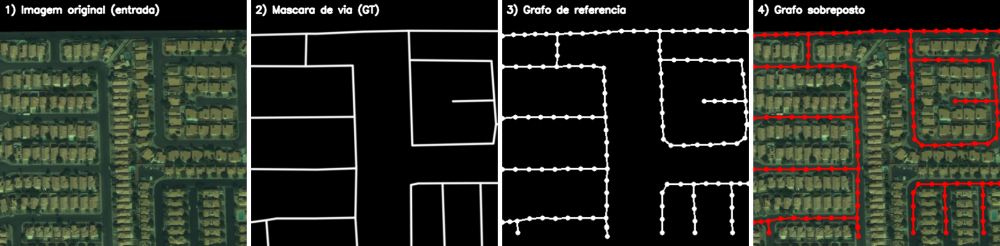
\includegraphics[width=\textwidth]{dataset_exemplo.png}
    \caption{Exemplo de um tile do SpaceNet 3: a imagem original (entrada) vem primeiro, seguida da máscara de via e do grafo de referência. As máscaras binárias não contêm rótulo asfalto/terra --- essa distinção é feita por heurística (Seção 4.6).}
    \label{fig:dataset}
\end{figure}

\subsection{Sobre o ajuste fino (não realizado)}

O dataset acima foi preparado para refinar os pesos do modelo no domínio
brasileiro. Entretanto, não foi possível executar o ajuste fino
por restrições de hardware: não dispomos de GPU local (a inferência roda em
CPU) e o Google Colab gratuito limita cada sessão de treino a
$\sim$4\,h, insuficiente para o ajuste completo do \textit{Vision Transformer}.
Portanto, todos os resultados deste relatório usam os pesos públicos
pré-treinados, sem ajuste fino. Mantemos a documentação e as capturas de tela
do dataset por completude e como base para trabalho futuro
(Seção~\ref{sec:futuro}).

\section{Metodologia}

O sistema é orquestrado por \texttt{run.py} (ou \texttt{processar\_pasta.py}
para uma pasta inteira). A imagem de entrada percorre nove etapas, ilustradas
nas Figuras~\ref{fig:passos1}--\ref{fig:passos3} para uma imagem urbana
representativa.

\subsection{Passo 1--2: pré-processamento e inferência multi-escala}

A imagem recebe um realce \texttt{canny\_fusion} (mistura de 15\% do mapa de
bordas de Canny), que destaca as bordas paralelas das vias. Esse realce
alimenta apenas a rede neural --- a classificação de pavimento, as máscaras e o
desenho final usam sempre a imagem original (bordas sintéticas não
podem ser confundidas com terra).

Em seguida, o codificador SAM ViT-B processa a imagem em janelas de
$512\times512$ com 50\% de sobreposição, em duas escalas, decididas por
uma passada rápida (\textit{scout}) que estima a largura típica das vias: zoom
alto usa 0{,}5$\times$ + 1{,}0$\times$; zoom padrão/distante usa 1{,}0$\times$ +
2{,}0$\times$ --- o aumento de escala de 2$\times$ é o que permite enxergar
estradas de terra muito finas. A fusão por máximo preserva tanto conexões finas
quanto largas. Há ainda \textit{test-time augmentation} opcional de rotação
(\texttt{--tta}).

\begin{figure}[H]
    \centering
    \begin{subfigure}[b]{0.32\textwidth}
        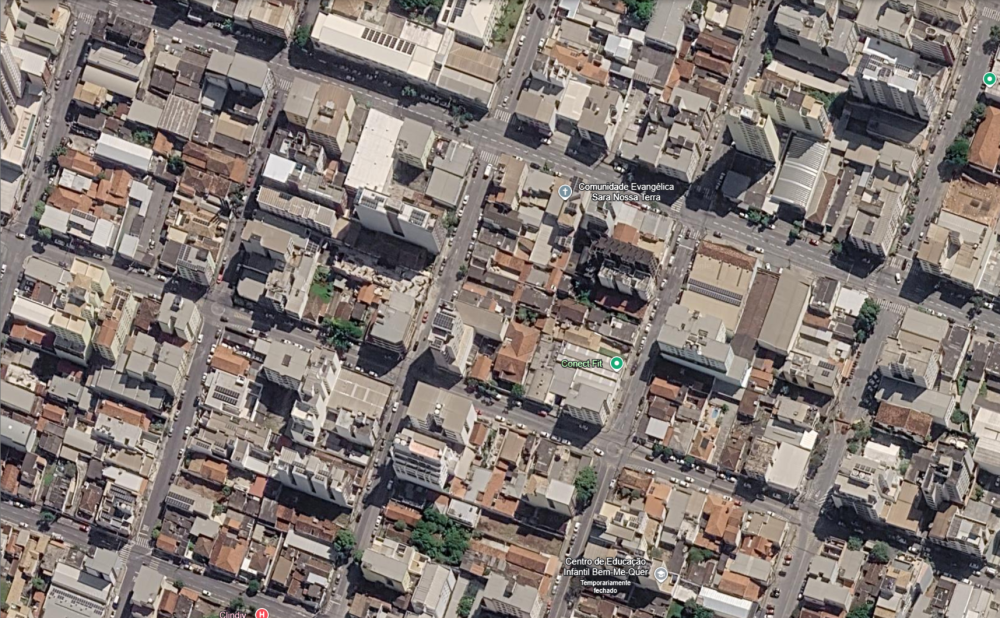
\includegraphics[width=\textwidth]{passo_1.png}\caption{Original}
    \end{subfigure}\hfill
    \begin{subfigure}[b]{0.32\textwidth}
        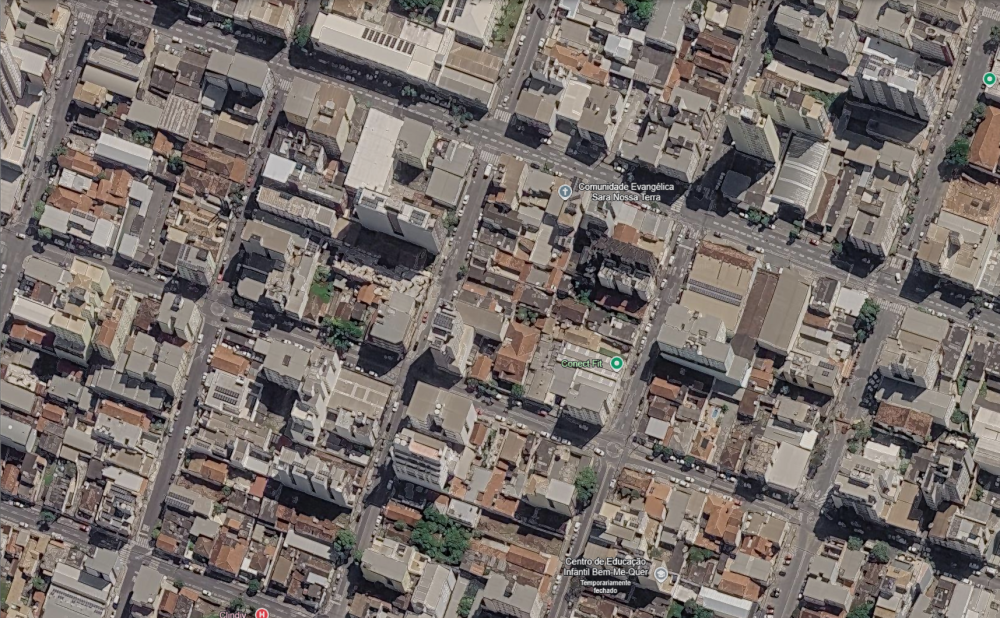
\includegraphics[width=\textwidth]{passo_2.png}\caption{Pré-proc.\ (canny)}
    \end{subfigure}\hfill
    \begin{subfigure}[b]{0.32\textwidth}
        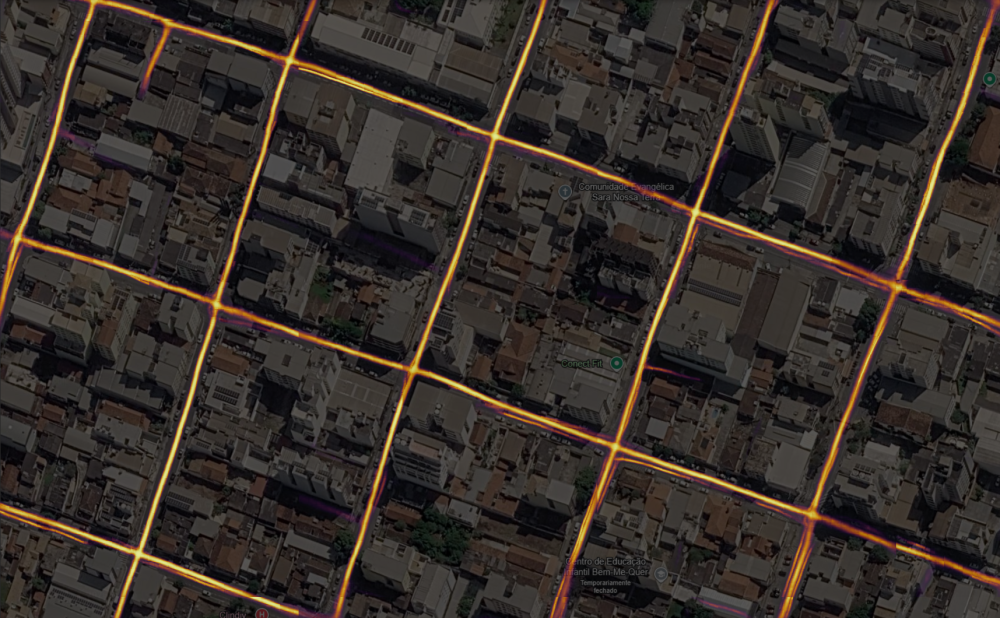
\includegraphics[width=\textwidth]{passo_3.png}\caption{Prob.\ de via (rede)}
    \end{subfigure}
    \caption{Passos 1--3: imagem original, realce de bordas e mapa de
    probabilidade de via produzido pela rede.}
    \label{fig:passos1}
\end{figure}

\subsection{Passo 3: máscaras de contexto}

O módulo \texttt{context\_filter.py} detecta quatro tipos de falso positivo e
suprime a probabilidade dessas regiões antes da binarização. A
visualização de depuração usa a codificação de cores da
Tabela~\ref{tab:cores}.

\begin{table}[H]
\centering
\caption{Codificação de cores da máscara de contexto (\texttt{context\_masks}).}
\label{tab:cores}
\begin{tabular}{@{}lll@{}}
\toprule
\textbf{Cor} & \textbf{Máscara} & \textbf{O que é} \\ \midrule
\textcolor{ForestGreen}{\textbf{Verde}}   & \texttt{vegetation}    & vegetação (floresta, mato, capim) \\
\textcolor{blue}{\textbf{Azul}}           & \texttt{water}         & água (rio, lago, mar) \\
\textcolor{red}{\textbf{Vermelho}}        & \texttt{roof}          & telhado / quarteirão (regiões construídas) \\
\textcolor{Dandelion}{\textbf{Amarelo}}   & \texttt{soil}          & solo exposto / desmatamento \\
\textcolor{Magenta}{\textbf{Rosa (magenta)}} & \texttt{bright\_reject} & vias claras rejeitadas (portão de brilho) \\ \bottomrule
\end{tabular}
\end{table}

As máscaras são calculadas a partir de heurísticas de cor, textura e morfologia matemática:
\begin{itemize}
    \item \textbf{Vegetação} (\texttt{vegetation}): É calculada por meio do índice de excesso de verde (\textit{Excess Green Index}, $ExG = 2G - R - B$). Para compensar variações na iluminação e na câmera, aplica-se uma correção de véu de cor global (color cast) que normaliza o matiz geral. Adicionalmente, faixas específicas do espaço de cores HSV são utilizadas para detectar vegetações secas ou claras que não possuem contraste de verde proeminente.
    \item \textbf{Água} (\texttt{water}): Baseia-se na ausência de textura de alta frequência (medida pelo desvio-padrão local de tons de cinza em uma vizinhança $5\times5$ inferior a um limiar) combinado com matizes frias no espaço HSV (azul/ciano escuro). Apenas componentes conectados de grande escala (área $\ge 3000$ pixels) são considerados, evitando confundir sombras de prédios com corpos d'água.
    \item \textbf{Telhado/quarteirão} (\texttt{roof}): Identifica telhados residenciais combinando componentes de cores quentes e claras, filtrando por morfologia para remover formas excessivamente alongadas (área $\ge 150$ pixels, razão de aspecto largura/altura $< 4$, garantindo formas 2-D). As sombras dos prédios, extraídas via limiarização de Otsu sobre o canal V, são incorporadas para consolidar a delimitação física dos lotes. Aplica-se então a regra dos quarteirões: se um polígono da máscara (estimado pelo seu fecho convexo ou convex hull) possui menos de 15\% de vazios internos (calculados sobre a área passível de preenchimento, ou seja, excluindo vias, vegetação e corpos d'água previamente identificados), o polígono é totalmente preenchido. Isso fecha buracos de sombra no interior de quarteirões residenciais densos. Para evitar a supressão de vias legítimas que atravessam os blocos, as ruas detectadas e as regiões onde a probabilidade de via do modelo é alta são recortadas (subtraídas) dessa máscara.
    \item \textbf{Solo exposto} (\texttt{soil}): Identifica clareiras e áreas de terraplanagem mapeando tons terrosos (marrom, bege, amarelo queimado) no espaço HSV. Para evitar a eliminação de estradas de terra legítimas (que possuem a mesma assinatura espectral), calcula-se a elongação do esqueleto de cada componente conexo usando a razão $L^2/\text{Area}$ (onde $L$ é o comprimento do esqueleto e $\text{Area}$ é a área do componente). Estradas têm formato 1-D estreito e alongado ($L^2/\text{Area} \ge 6{,}0$), mantendo-se ativas, enquanto clareiras e descampados 2-D ($L^2/\text{Area} < 6{,}0$) são classificados como solo exposto e suprimidos.
    \item \textbf{Vias claras rejeitadas} (\texttt{bright\_reject}): Funciona como um portão de brilho que atua apenas em zooms urbanos próximos (fator de escala $\ge 14$\,px). Regiões com altíssima luminosidade (canal V $\ge 205$) e baixa saturação são mascaradas para evitar que reflexos solares em telhados de zinco ou portões metálicos causem falsos positivos de asfalto.
\end{itemize}

Pixels onde a rede tem alta confiança nunca são suprimidos (ex.: ponte sobre rio). Telhado e solo usam supressão suave (mantêm um resíduo), para que um trecho de rua fraco que caia sobre eles sobreviva.

\subsection{Detecção automática de domínio: urbano vs.\ rural}

Todo o refino do grafo (adiante) é calibrado para malha urbana; em
cenário rural/florestal ele distorce. O sistema decide o domínio
automaticamente: é rural quando há muita vegetação ($>25\%$)
e malha viária esparsa ($<1{,}2\%$ da imagem). A vegetação sozinha não basta
--- uma favela num vale verde tem $40\%+$ de verde mas malha
densa, e é urbana. A densidade da via separa os domínios de forma
limpa (rural de verdade $\le 0{,}6\%$; favela/urbano $\ge 2\%$). Em imagem
rural, o refino é pulado, as máscaras de telhado/solo são desligadas (só
vegetação + água suprimem) e o limiar de terra é baixo (mais terra).

\subsection{Passos 4--5: binarização e grafo}

A binarização por histerese (hysteresis binarization) é empregada sobre a probabilidade suprimida para mitigar falhas de conectividade (efeito de quebras causadas por sombras ou copas de árvores). O processo utiliza dois limiares distintos: um limiar alto (semente ou seed) de $0{,}30$ e um limiar baixo (crescimento ou growth) de $0{,}04$. Um pixel é ativado se o seu valor de probabilidade for superior ao limiar alto, ou se estiver conectado a um pixel já ativado e seu valor for superior ao limiar baixo.

Para lidar com imagens fora do domínio de treinamento do modelo, onde o sinal de probabilidade retornado pela rede pode ser globalmente muito fraco, o algoritmo adota um regime adaptativo de sinal fraco. Caso o pico de probabilidade na imagem inteira seja inferior a $0{,}30$ (porém acima de um piso mínimo de $0{,}10$), os limiares são reajustados dinamicamente em relação ao valor máximo observado ($\text{max\_prob}$):
\begin{align}
\text{limiar\_alto} &= 0{,}45 \times \text{max\_prob} \\
\text{limiar\_baixo} &= 0{,}12 \times \text{max\_prob}
\end{align}
Essa adaptação dinâmica preserva o contorno das vias mesmo sob forte atenuação do sinal. Após a binarização, a máscara binária é submetida a uma operação de esqueletização (skeletonization) por afinamento morfológico para obter linhas de 1 pixel de espessura. Esse esqueleto é convertido em um grafo bruto (\texttt{graph\_refine.py}) onde os nós correspondem a interseções (cruzamentos) ou terminações (pontas soltas), e as arestas representam os segmentos de via (polylines).

\begin{figure}[H]
    \centering
    \begin{subfigure}[b]{0.32\textwidth}
        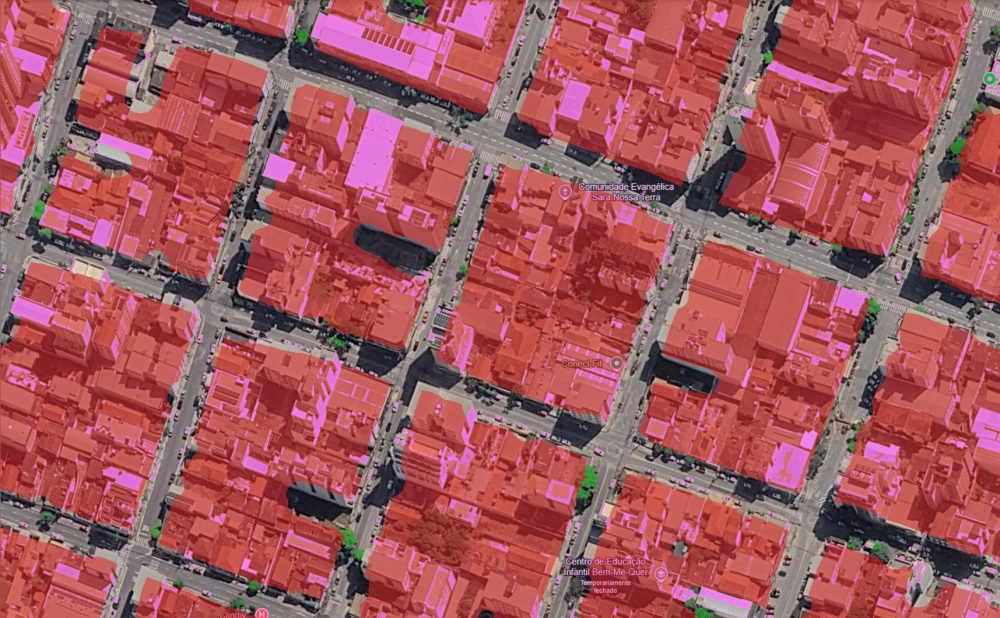
\includegraphics[width=\textwidth]{passo_4.png}\caption{Máscaras de contexto}
    \end{subfigure}\hfill
    \begin{subfigure}[b]{0.32\textwidth}
        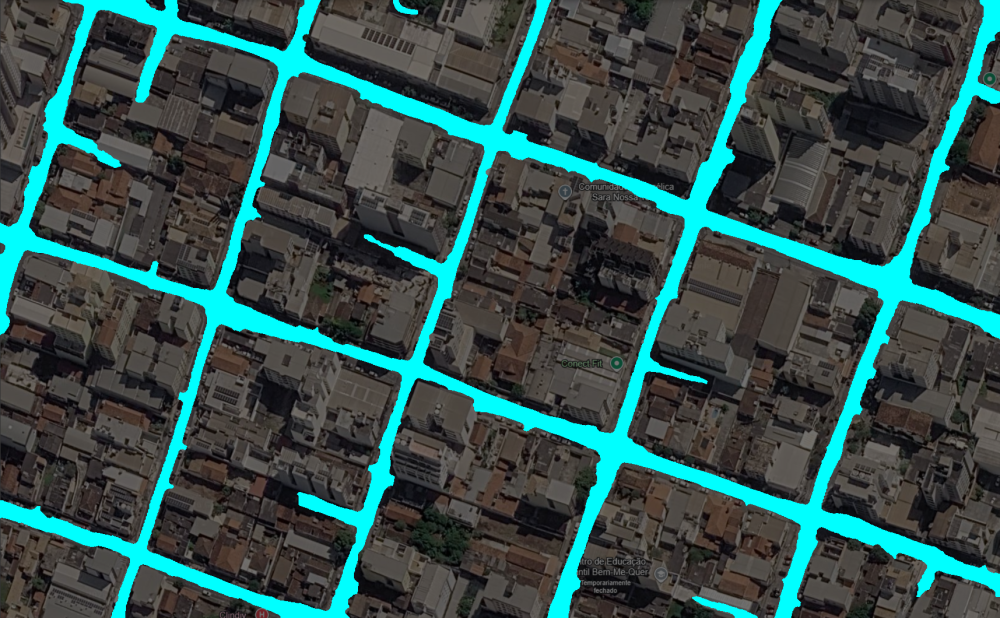
\includegraphics[width=\textwidth]{passo_6.png}\caption{Binária (hysteresis)}
    \end{subfigure}\hfill
    \begin{subfigure}[b]{0.32\textwidth}
        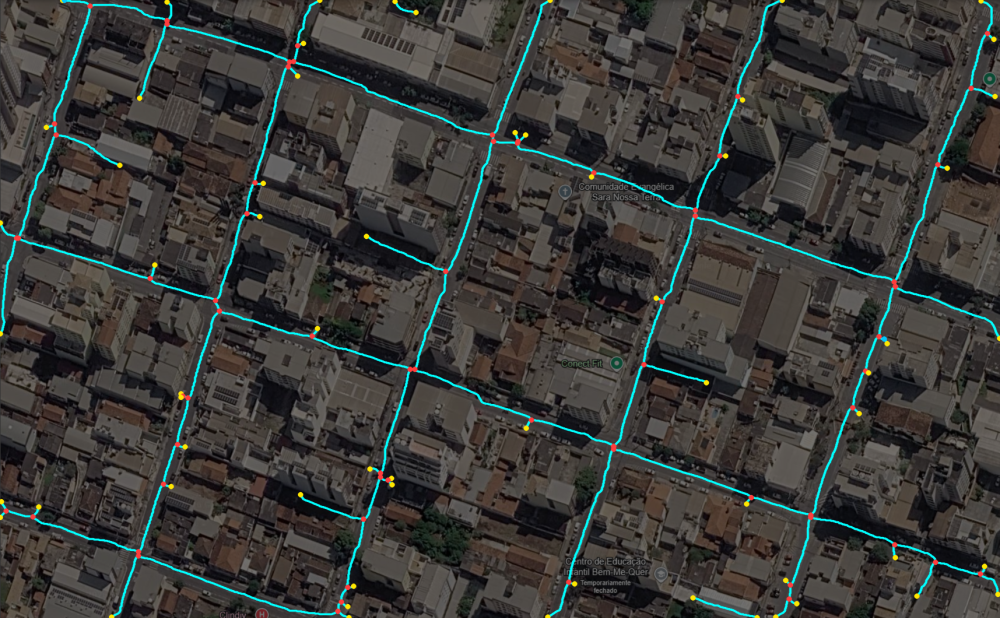
\includegraphics[width=\textwidth]{passo_7.png}\caption{Grafo bruto}
    \end{subfigure}
    \caption{Passos 3--4: máscaras de contexto (cores da Tabela~\ref{tab:cores}),
    máscara binária e grafo bruto (vermelho = cruzamentos; amarelo = pontas).}
    \label{fig:passos2}
\end{figure}

\subsection{Passo 5: refino do grafo (fonte única de verdade)}

O esqueleto gerado costuma conter diversas imperfeições topológicas (falsas junções duplicadas, pontas soltas devido a oclusões e traços espúrios em telhados ou sombras). O módulo \texttt{graph\_refine.py} realiza as correções de forma puramente topológica sobre o grafo:
\begin{itemize}
    \item \textbf{Fusão de nós duplicados de junções}: Devido à espessura residual na binarização, cruzamentos reais frequentemente geram nós duplicados muito próximos. Nós cuja distância mútua seja inferior a $0{,}8 \times \text{largura\_típica}$ da via são fundidos em um único vértice centralizado, simplificando a topologia da junção.
    \item \textbf{Poda de pontas curtas (stubs)}: Pontas soltas (arestas de grau 1) com comprimento inferior à largura típica da estrada são eliminadas, pois representam ruídos da binarização. Adicionalmente, qualquer ponta solta cuja terminação espacial caia dentro de um polígono classificado como telhado (\texttt{roof}) é imediatamente podada (``via dentro de casa''), pois indica falso positivo de via avançando sobre residências.
    \item \textbf{Pontes Dijkstra em buracos de sinal}: Para reconectar trechos de via interrompidos sob copas de árvores ou sombras longas, realiza-se uma busca direcional de menor custo usando o algoritmo de Dijkstra entre pontas soltas orientadas. O grafo implícito de pixels usa a função de custo:
    \begin{equation}
    \text{Custo} = \frac{1}{\text{probabilidade\_via}} + \text{custo\_contexto}
    \end{equation}
    Neste cálculo, pixels de água ou telhado agem como obstáculos intransponíveis (custo infinito). A vegetação encarece significativamente o caminho (reduzindo a chance de conexões errôneas), mas não o bloqueia inteiramente, permitindo que a busca reconecte as pontas se houver um sinal residual coerente de via sob a copa.
    \item \textbf{Remoção de traços internos de quarteirão (block stubs)}: Uma rua que entra em um quarteirão e termina sem saída (aresta com uma ponta solta de grau 1) é candidata a ruído de sombra ou vão entre casas. O algoritmo calcula o retângulo envolvente (bounding box) do bloco residencial circundante. Se o comprimento dessa aresta sem saída for inferior a 80\% da menor dimensão lateral desse retângulo ($0{,}8 \times \text{lado\_menor}$), a aresta e sua terminação são eliminadas.
\end{itemize}

\textbf{Limitação e Tolerância em Áreas Rurais}: Todo o pipeline de refino topológico do grafo (incluindo fusão, Dijkstra e podas internas de quarteirão) é projetado para padrões urbanos e residenciais densos. Em áreas rurais ou de floresta densa (definidas automaticamente na detecção de domínio quando a vegetação excede 25\% e a densidade de vias na imagem é inferior a 1,2\%), o refino topológico é completamente contornado (ignorado). Esse bypass evita que o Dijkstra trace linhas retas incorretas entre estradas rurais isoladas ou que podas morfológicas urbanas eliminem acessos reais de fazendas que terminam de forma abrupta.

\subsection{Passo 6: classificação de pavimento por aresta}
\label{sec:classif}

Em vez de decidir pixel a pixel (que causa efeito ``zebra''), a classe é
decidida por aresta inteira: a mediana da evidência de cor/textura ao
longo do núcleo da via. A evidência combina matiz quente HSV (terra é
marrom/laranja) e desvio-padrão local (terra é granular; asfalto é liso). O
limiar terra$\times$asfalto é adaptativo por domínio: imagem urbana usa
limiar alto (evita asfalto fino virar laranja); rural usa limiar baixo (pega
estrada de terra), pois terra seca clara e asfalto cinza ficam próximos nessa
evidência. Uma suavização tipo Potts (ICM) faz vias contínuas compartilharem a
classe, e um trecho de terra cercado só por asfalto é revertido para asfalto.
Terra = laranja; asfalto = azul.

\begin{figure}[H]
    \centering
    \begin{subfigure}[b]{0.48\textwidth}
        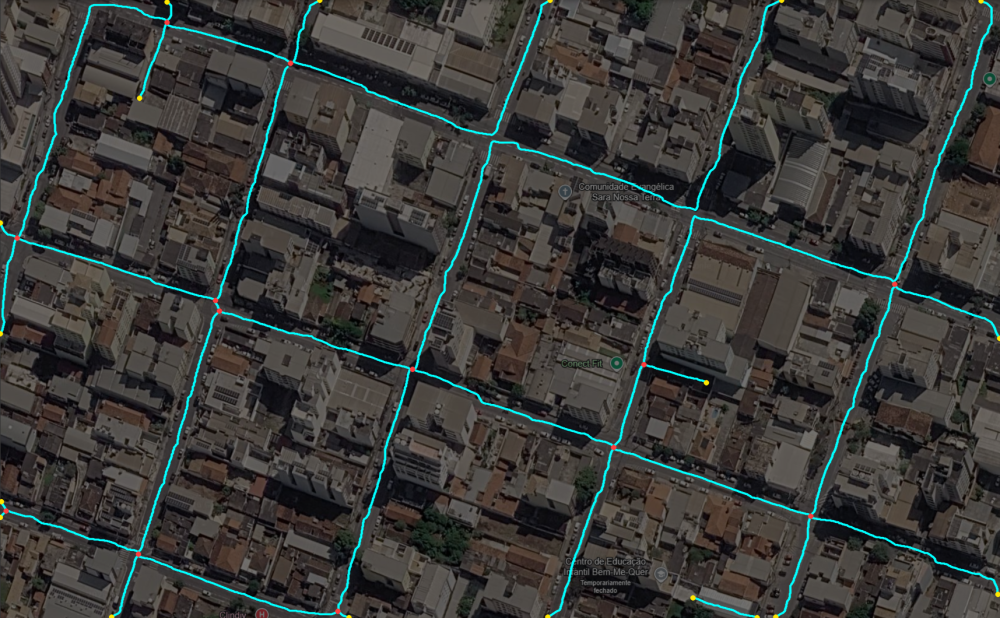
\includegraphics[width=\textwidth]{passo_8.png}\caption{Grafo refinado}
    \end{subfigure}\hfill
    \begin{subfigure}[b]{0.48\textwidth}
        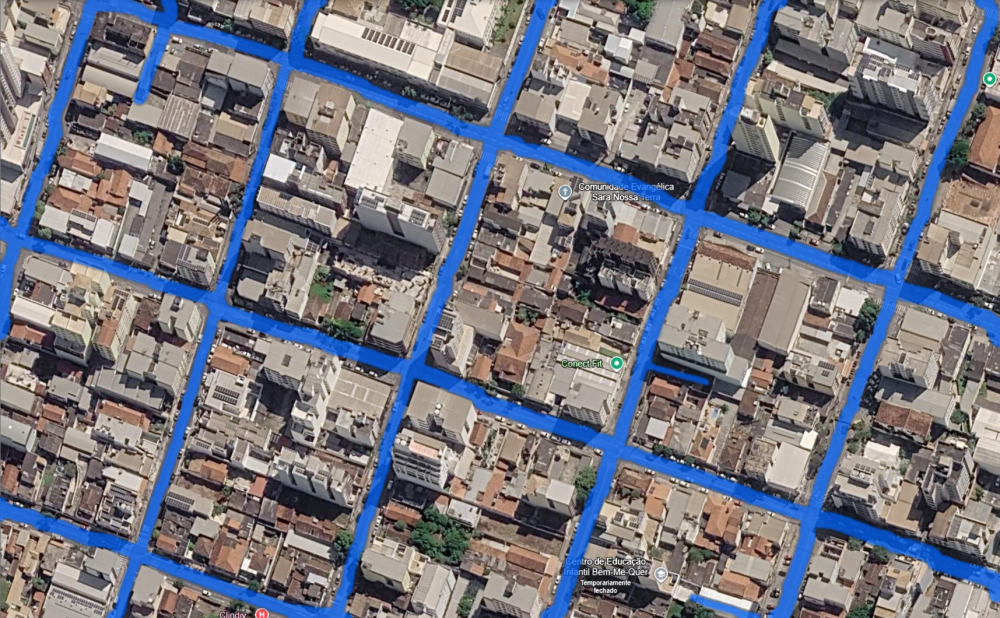
\includegraphics[width=\textwidth]{passo_9.png}\caption{Overlay final}
    \end{subfigure}
    \caption{Passos 5--6: grafo refinado e sobreposição final (azul =
    asfalto, laranja = terra).}
    \label{fig:passos3}
\end{figure}

\subsection{Saídas}

Por execução são gravados: a sobreposição (desenhada do grafo, com espessura
medida por transformada de distância), a máscara de classes, a máscara de
contexto e o grafo em JSON e GraphML (vértices, arestas, pavimento,
largura, comprimento, confiança).

\section{Resultados}

A avaliação quantitativa (\texttt{eval/run\_eval.py}, F1 de centerline com
margem (buffer) de 8\,px sobre o SpaceNet~3) mostra que o pós-processamento em
grafo eleva o F1 de $0{,}751$ (método pixel-a-pixel anterior) para
$0{,}909$ (mesmo modelo, mesmos mosaicos), com metade dos falsos
positivos. A seguir, a análise qualitativa nas sete imagens de teste
(Figuras~\ref{fig:res_2026-06-12_135241} a \ref{fig:res_2026-06-14_131959}).

\begin{table}[H]
\centering
\caption{Resumo qualitativo por imagem.}
\label{tab:resumo}
\footnotesize
\begin{tabular}{@{}p{3.2cm}p{2.0cm}p{8.5cm}@{}}
\toprule
\textbf{Imagem} & \textbf{Domínio} & \textbf{Avaliação} \\ \midrule
135241 & Urbano denso & \textbf{Perfeito}: cidade e quarteirões bem definidos. \\
003536 & Favela (verde) & \textbf{Perfeita} classificação; densamente residencial, quarteirões bem definidos, com muita vegetação nas bordas. \\
202053 (PDF prof.) & Rural & \textbf{Muito boa}; o \textit{print} já trazia marcação de vias em branco claro, o que facilitou a execução do algoritmo. \\
165358 & Rural & Melhorou bastante após a detecção de domínio; faltam algumas ruas de textura muito fraca (executada sem \texttt{--tta}). \\
020059 & Urbano & Quarteirões bem definidos, boa classificação; porém a \texttt{context\_masks} marcou vermelho sobre ruas, deixando algumas vias incompletas. \\
151237 & Favela (verde) & Média/boa; a \texttt{context\_masks} não reconheceu um telhado como telhado e marcou uma via sobre ele. \\
131959 & Rural & Funcionou bem, mas com ruas incompletas e várias vias sem marcar. \\ \bottomrule
\end{tabular}
\end{table}

\begin{figure}[H]
    \centering
    \begin{subfigure}[b]{0.24\textwidth}
        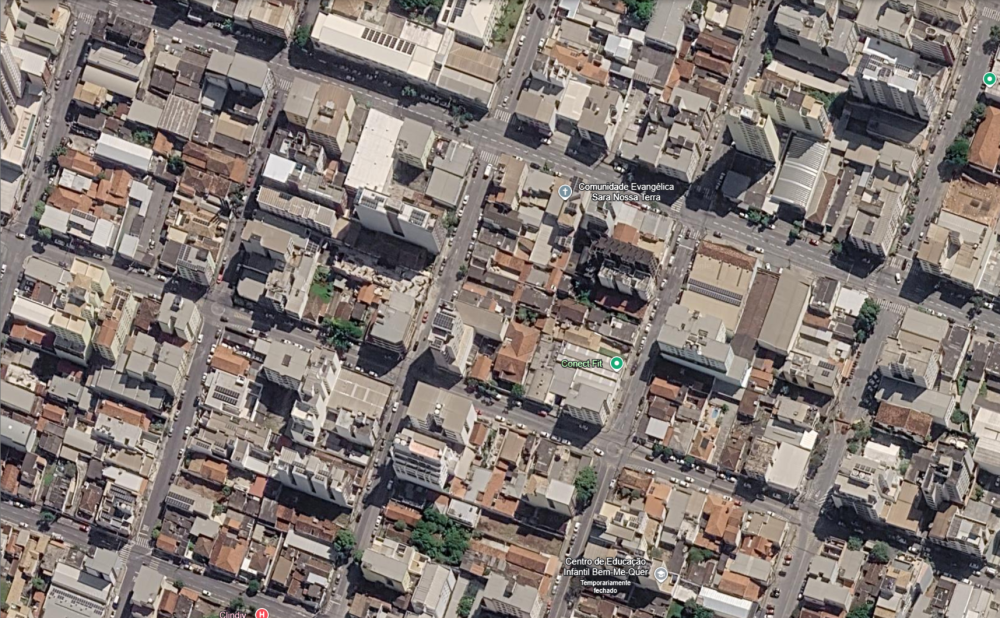
\includegraphics[width=\textwidth]{2026-06-12_135241_passo_1.png}
        \caption{Original}
    \end{subfigure}\hfill
    \begin{subfigure}[b]{0.24\textwidth}
        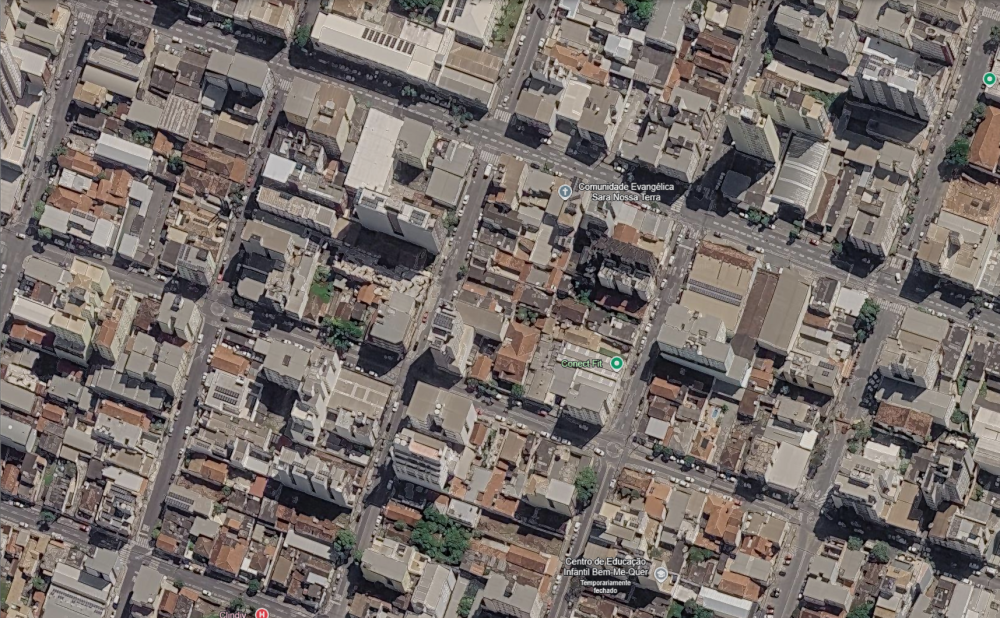
\includegraphics[width=\textwidth]{2026-06-12_135241_passo_2.png}
        \caption{Pré-proc.}
    \end{subfigure}\hfill
    \begin{subfigure}[b]{0.24\textwidth}
        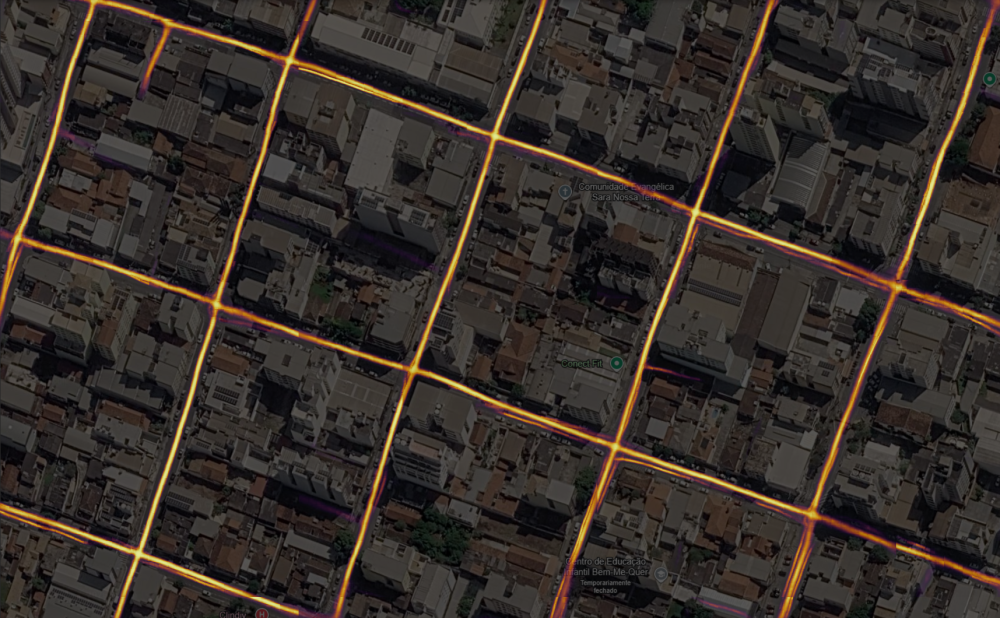
\includegraphics[width=\textwidth]{2026-06-12_135241_passo_3.png}
        \caption{Prob.\ Modelo}
    \end{subfigure}\hfill
    \begin{subfigure}[b]{0.24\textwidth}
        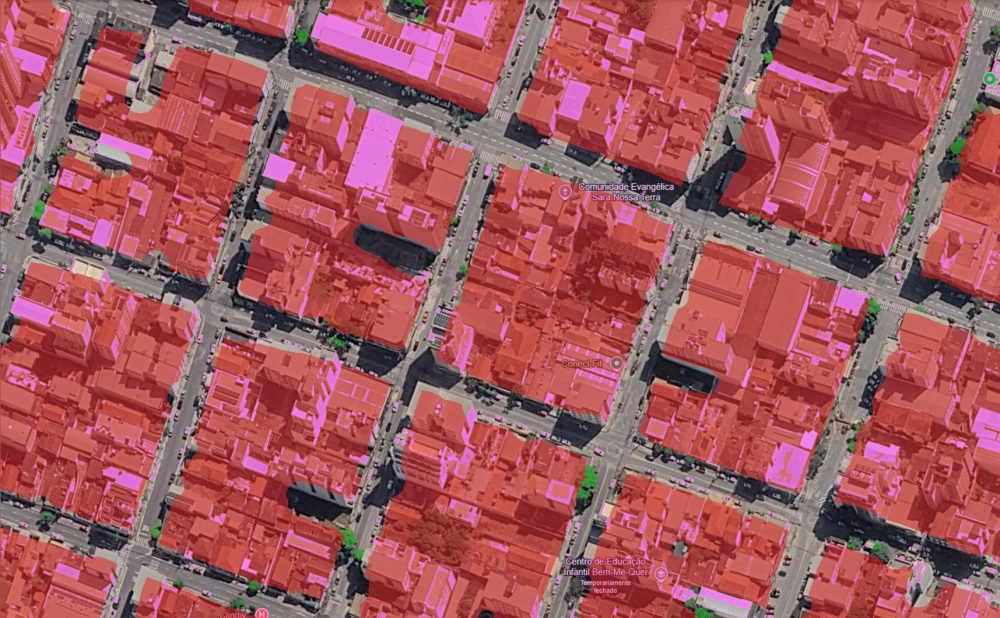
\includegraphics[width=\textwidth]{2026-06-12_135241_passo_4.png}
        \caption{Máscaras}
    \end{subfigure}
    
    \vspace{0.15cm}
    \begin{subfigure}[b]{0.24\textwidth}
        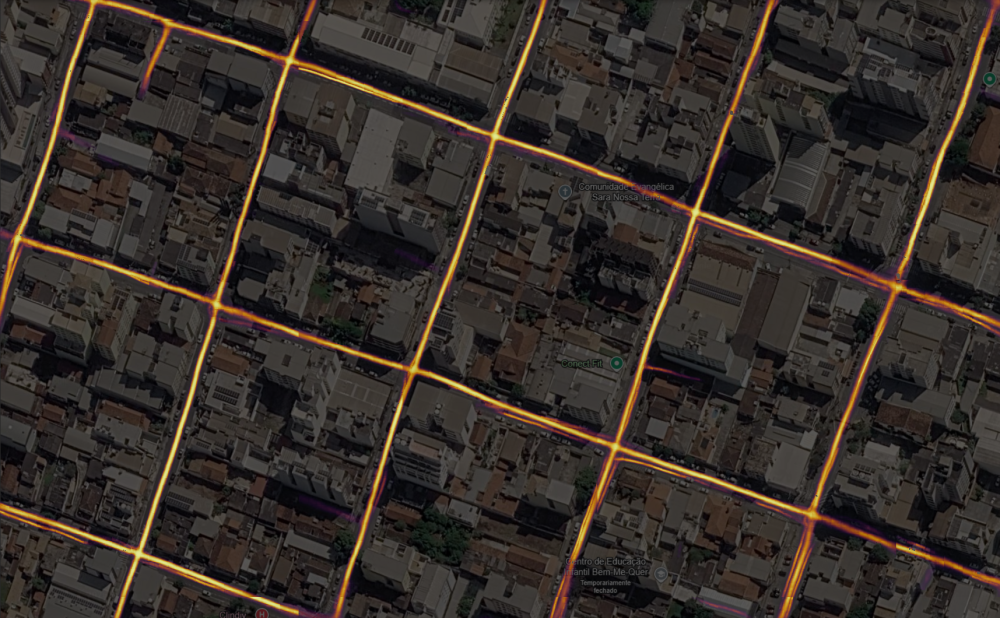
\includegraphics[width=\textwidth]{2026-06-12_135241_passo_5.png}
        \caption{Prob.\ Supr.}
    \end{subfigure}\hfill
    \begin{subfigure}[b]{0.24\textwidth}
        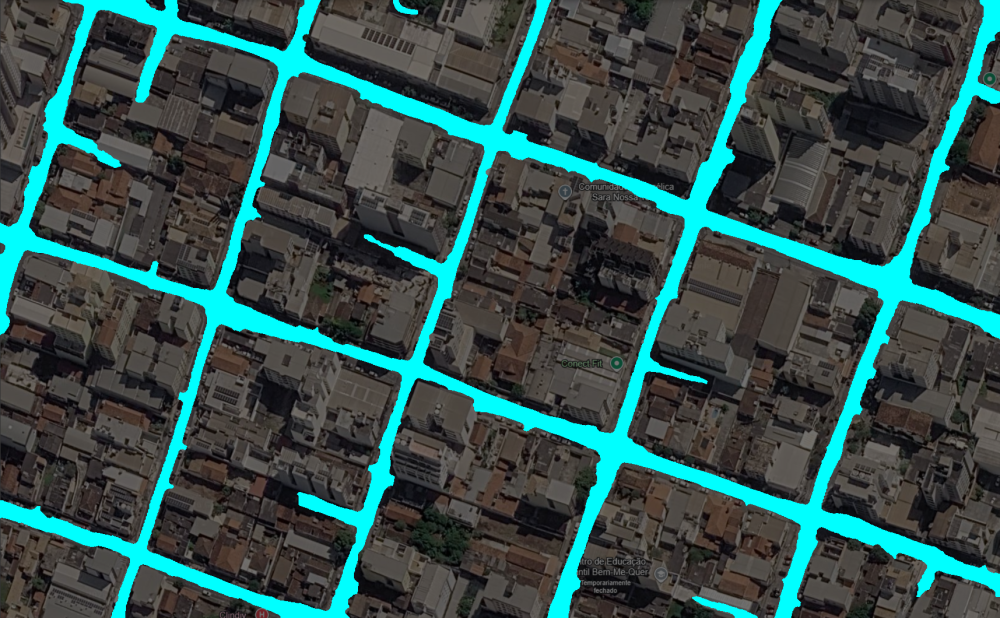
\includegraphics[width=\textwidth]{2026-06-12_135241_passo_6.png}
        \caption{Binária}
    \end{subfigure}\hfill
    \begin{subfigure}[b]{0.24\textwidth}
        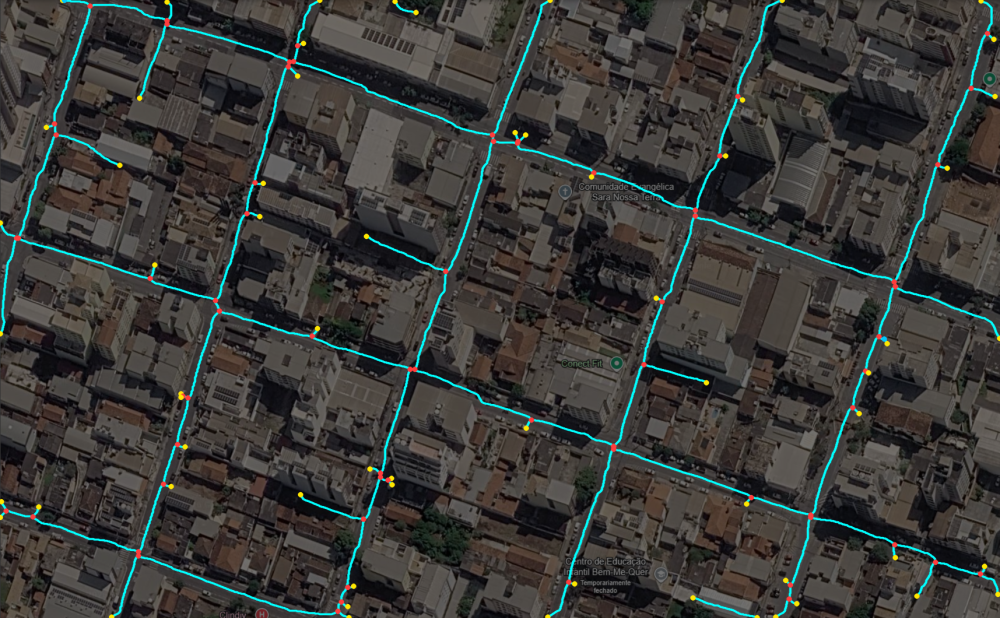
\includegraphics[width=\textwidth]{2026-06-12_135241_passo_7.png}
        \caption{Grafo Bruto}
    \end{subfigure}\hfill
    \begin{subfigure}[b]{0.24\textwidth}
        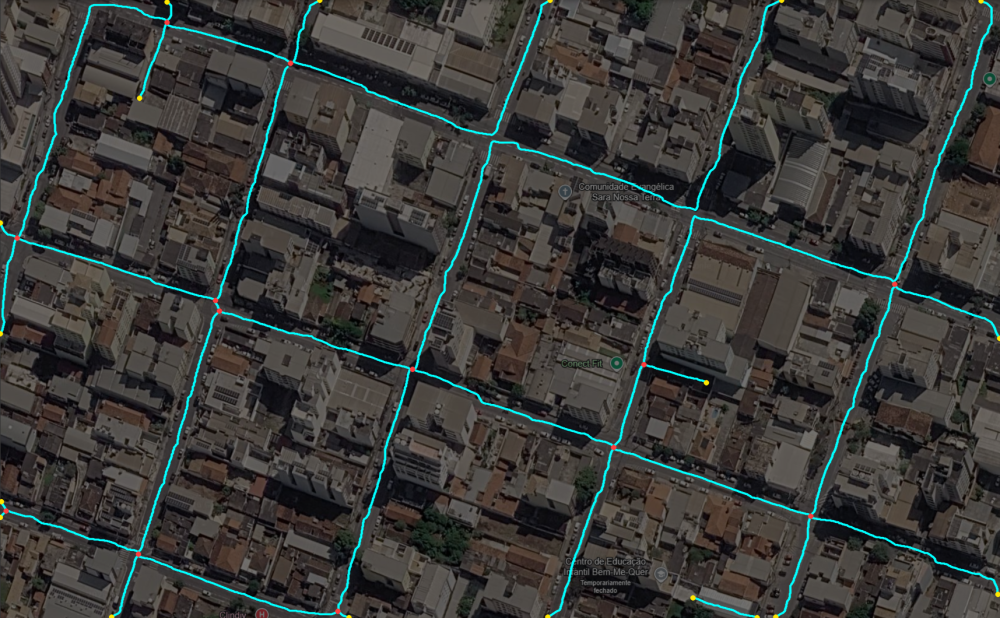
\includegraphics[width=\textwidth]{2026-06-12_135241_passo_8.png}
        \caption{Grafo Ref.}
    \end{subfigure}
    
    \vspace{0.15cm}
    \begin{subfigure}[b]{0.8\textwidth}
        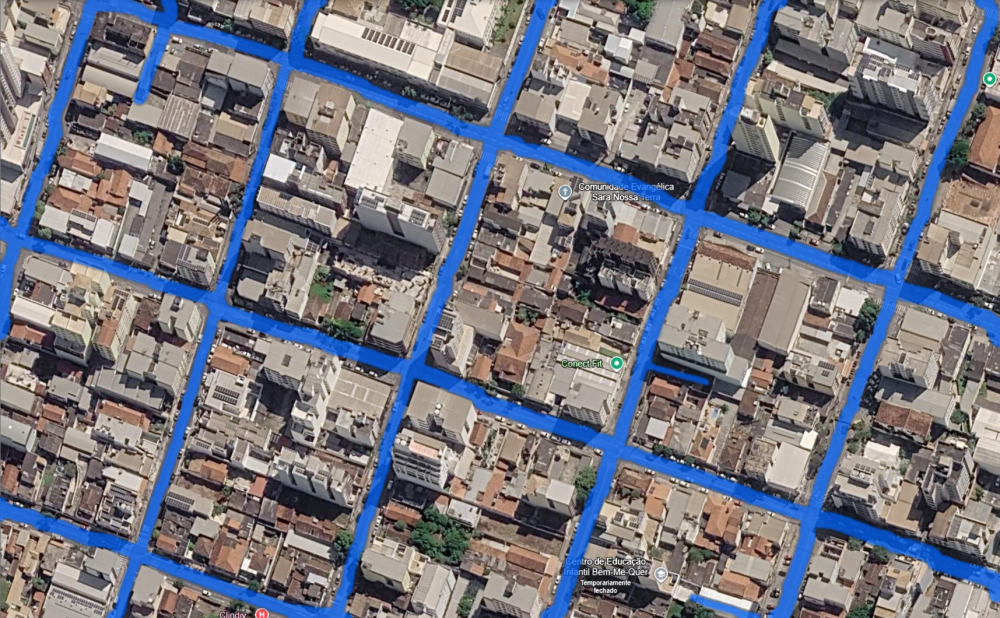
\includegraphics[width=\textwidth]{2026-06-12_135241_passo_9.png}
        \caption{Overlay final com pavimento classificado}
    \end{subfigure}
    \caption{Resultados do pipeline passo a passo para a imagem 135241 --- Urbano denso (cidade e quarteirões bem definidos).}
    \label{fig:res_2026-06-12_135241}
\end{figure}

\begin{figure}[H]
    \centering
    \begin{subfigure}[b]{0.24\textwidth}
        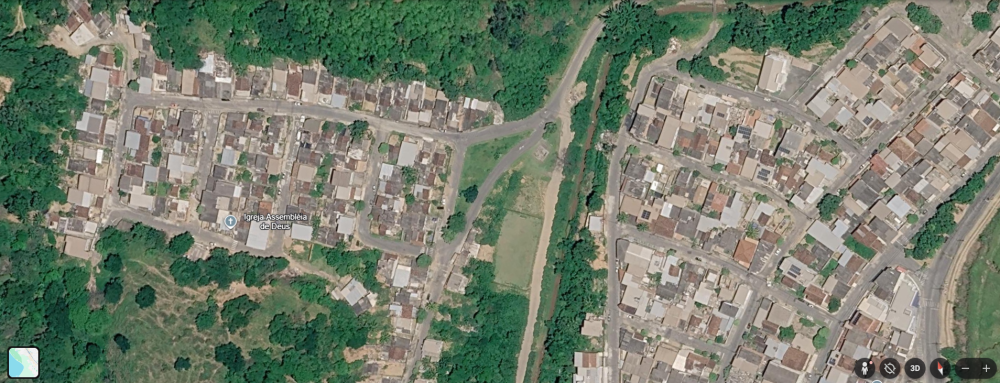
\includegraphics[width=\textwidth]{2026-05-12_003536_passo_1.png}
        \caption{Original}
    \end{subfigure}\hfill
    \begin{subfigure}[b]{0.24\textwidth}
        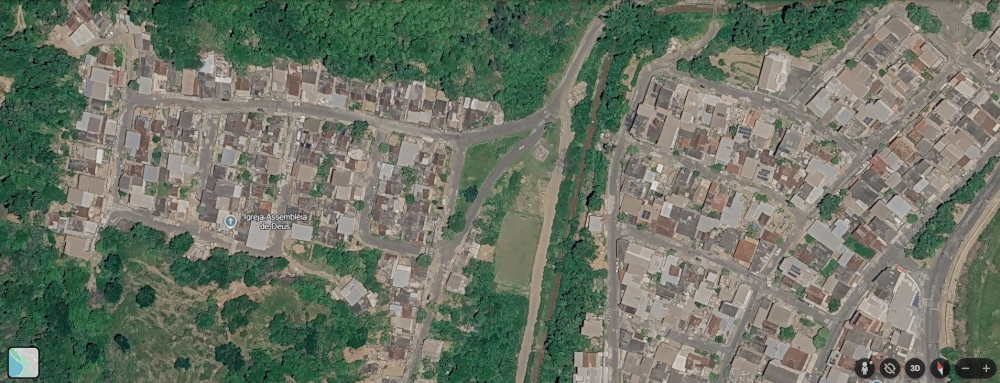
\includegraphics[width=\textwidth]{2026-05-12_003536_passo_2.png}
        \caption{Pré-proc.}
    \end{subfigure}\hfill
    \begin{subfigure}[b]{0.24\textwidth}
        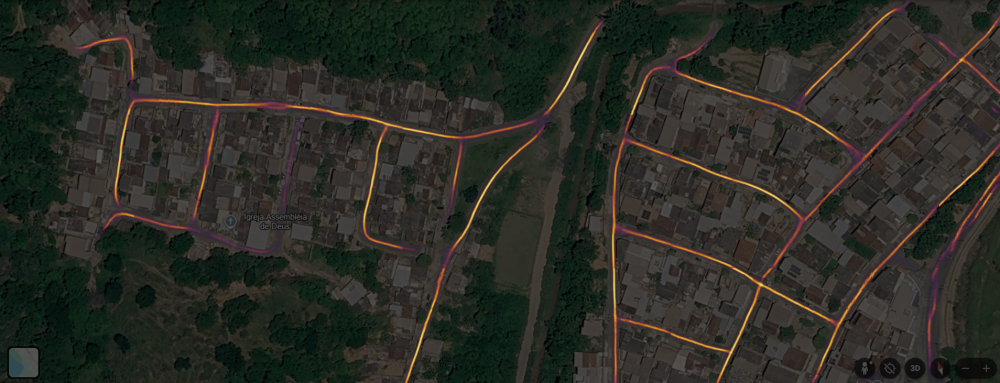
\includegraphics[width=\textwidth]{2026-05-12_003536_passo_3.png}
        \caption{Prob.\ Modelo}
    \end{subfigure}\hfill
    \begin{subfigure}[b]{0.24\textwidth}
        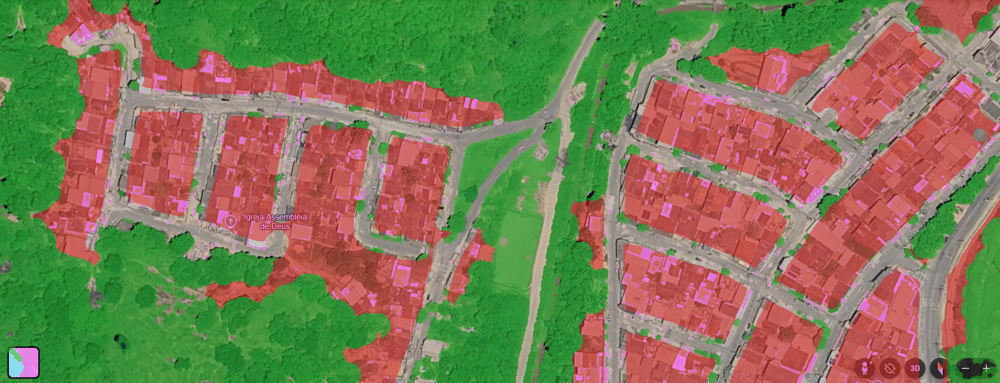
\includegraphics[width=\textwidth]{2026-05-12_003536_passo_4.png}
        \caption{Máscaras}
    \end{subfigure}
    
    \vspace{0.15cm}
    \begin{subfigure}[b]{0.24\textwidth}
        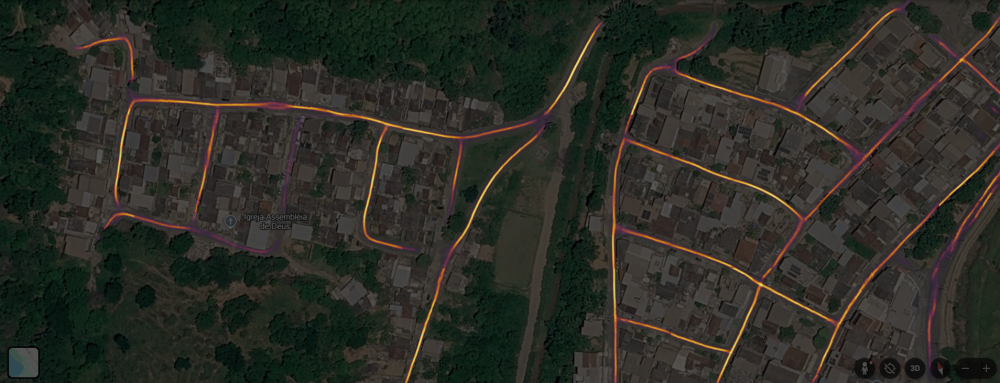
\includegraphics[width=\textwidth]{2026-05-12_003536_passo_5.png}
        \caption{Prob.\ Supr.}
    \end{subfigure}\hfill
    \begin{subfigure}[b]{0.24\textwidth}
        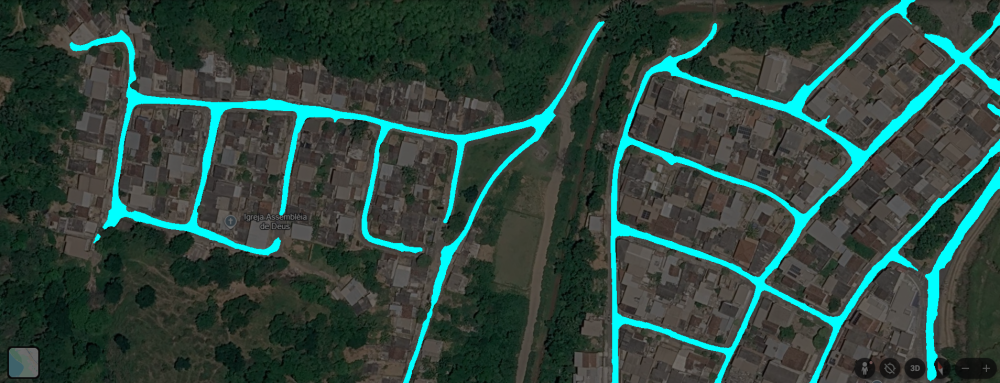
\includegraphics[width=\textwidth]{2026-05-12_003536_passo_6.png}
        \caption{Binária}
    \end{subfigure}\hfill
    \begin{subfigure}[b]{0.24\textwidth}
        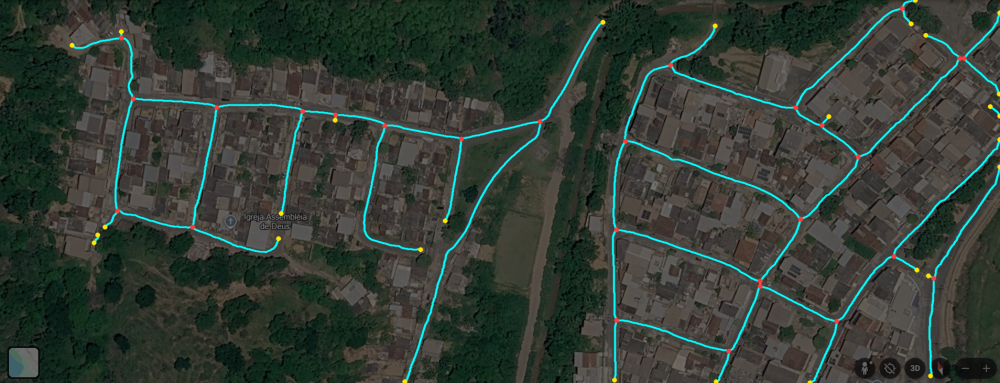
\includegraphics[width=\textwidth]{2026-05-12_003536_passo_7.png}
        \caption{Grafo Bruto}
    \end{subfigure}\hfill
    \begin{subfigure}[b]{0.24\textwidth}
        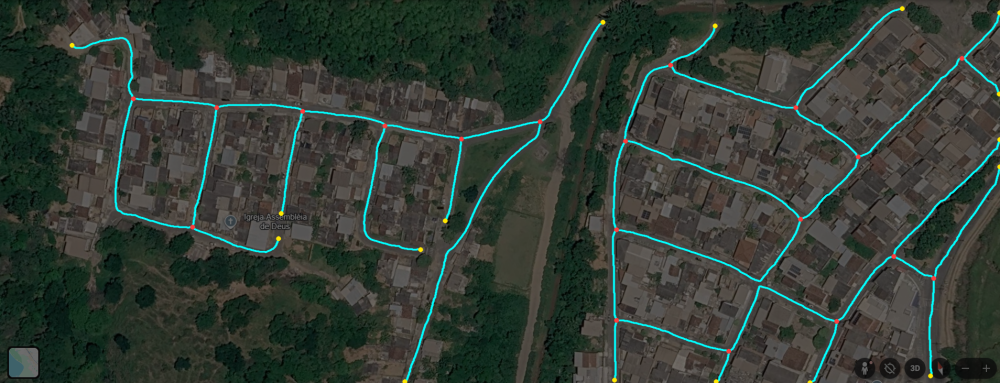
\includegraphics[width=\textwidth]{2026-05-12_003536_passo_8.png}
        \caption{Grafo Ref.}
    \end{subfigure}
    
    \vspace{0.15cm}
    \begin{subfigure}[b]{0.8\textwidth}
        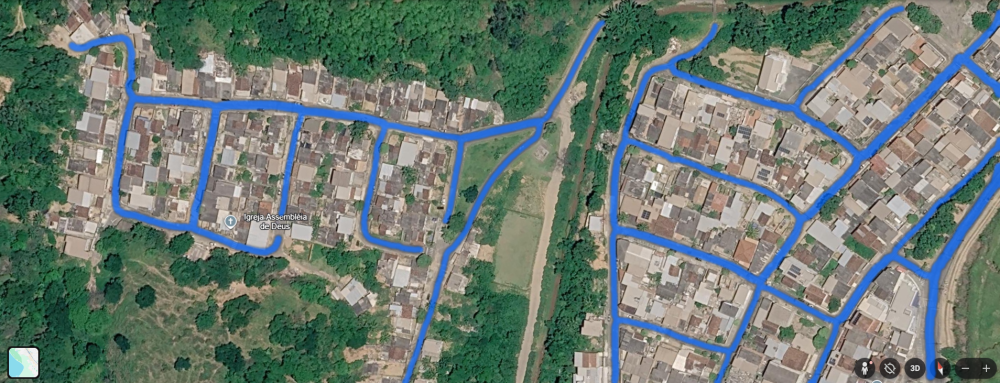
\includegraphics[width=\textwidth]{2026-05-12_003536_passo_9.png}
        \caption{Overlay final com pavimento classificado}
    \end{subfigure}
    \caption{Resultados do pipeline passo a passo para a imagem 003536 --- Favela em vale verde (área residencial densa, quarteirões consolidados).}
    \label{fig:res_2026-05-12_003536}
\end{figure}

\begin{figure}[H]
    \centering
    \begin{subfigure}[b]{0.24\textwidth}
        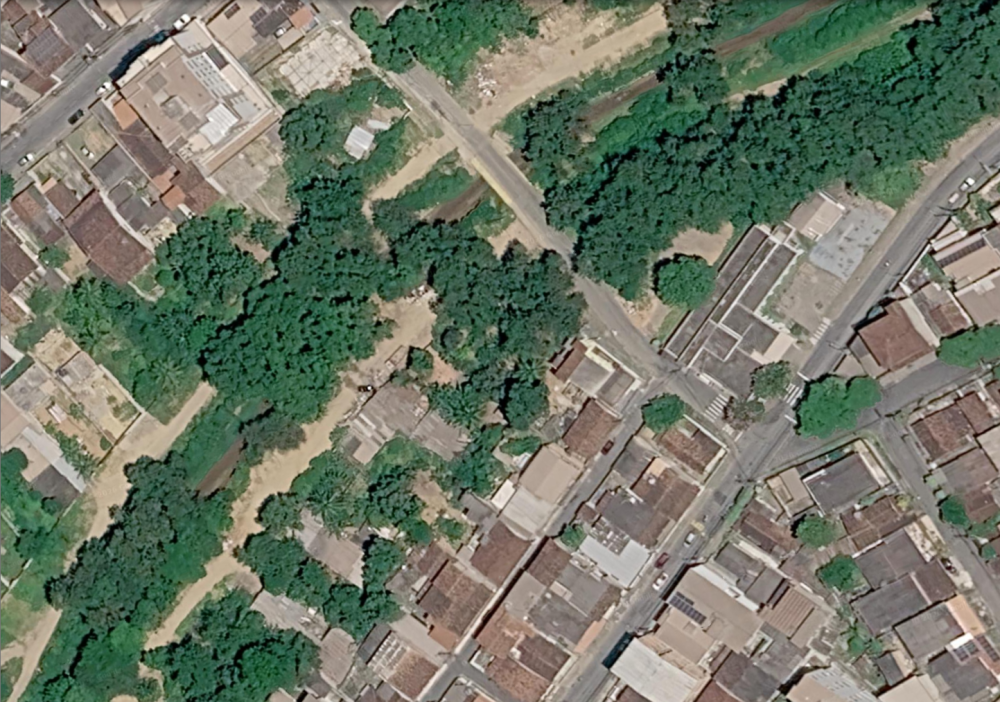
\includegraphics[width=\textwidth]{2026-05-12_151237_passo_1.png}
        \caption{Original}
    \end{subfigure}\hfill
    \begin{subfigure}[b]{0.24\textwidth}
        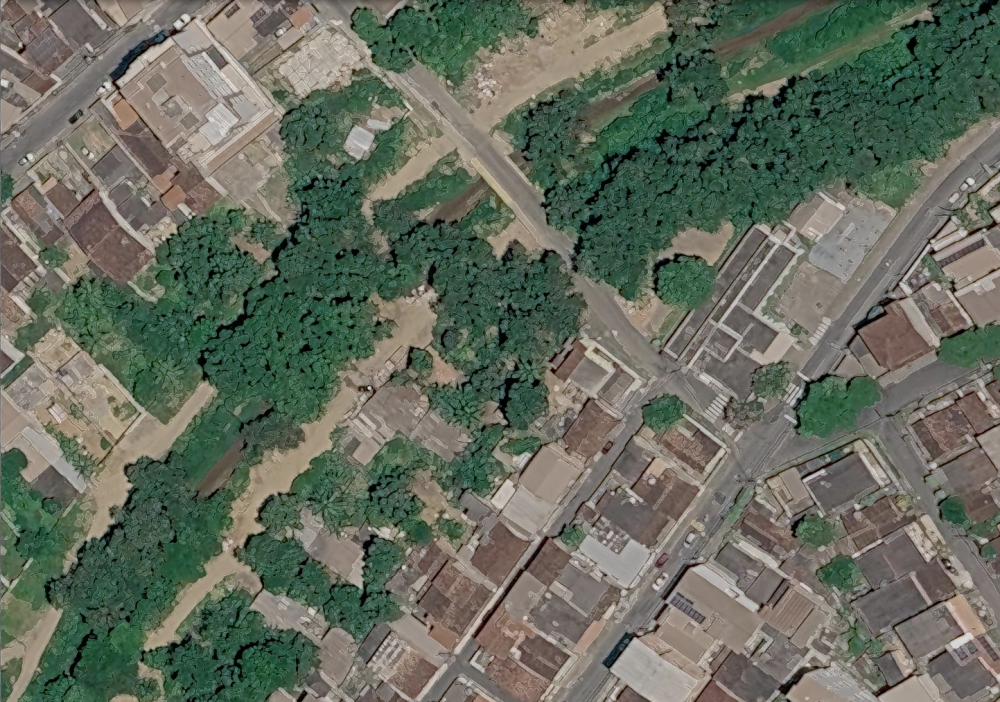
\includegraphics[width=\textwidth]{2026-05-12_151237_passo_2.png}
        \caption{Pré-proc.}
    \end{subfigure}\hfill
    \begin{subfigure}[b]{0.24\textwidth}
        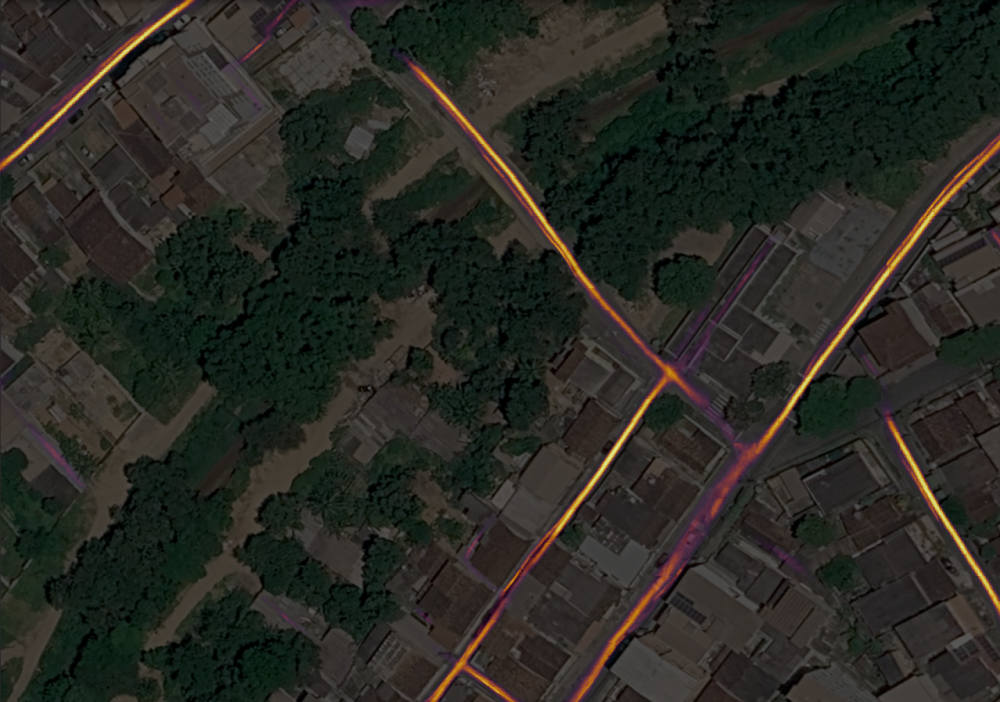
\includegraphics[width=\textwidth]{2026-05-12_151237_passo_3.png}
        \caption{Prob.\ Modelo}
    \end{subfigure}\hfill
    \begin{subfigure}[b]{0.24\textwidth}
        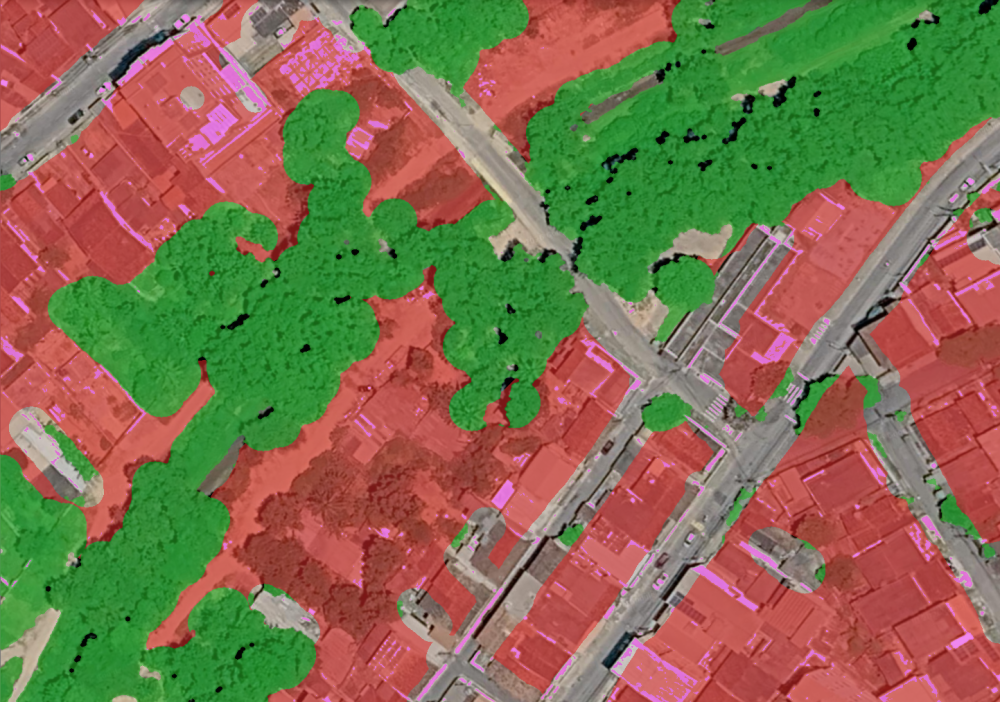
\includegraphics[width=\textwidth]{2026-05-12_151237_passo_4.png}
        \caption{Máscaras}
    \end{subfigure}
    
    \vspace{0.15cm}
    \begin{subfigure}[b]{0.24\textwidth}
        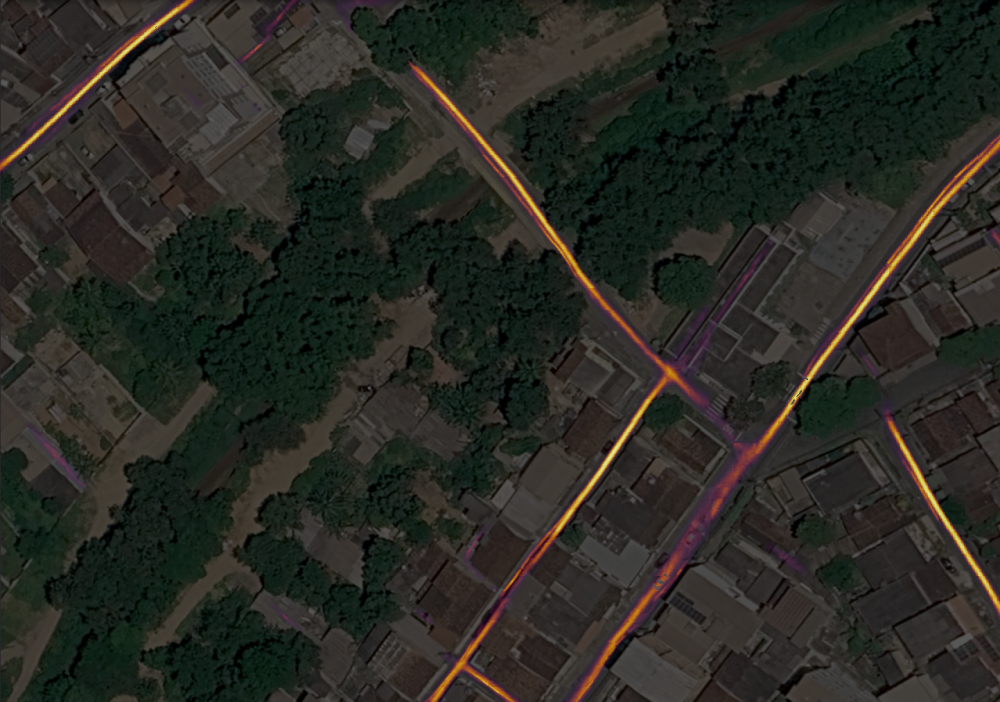
\includegraphics[width=\textwidth]{2026-05-12_151237_passo_5.png}
        \caption{Prob.\ Supr.}
    \end{subfigure}\hfill
    \begin{subfigure}[b]{0.24\textwidth}
        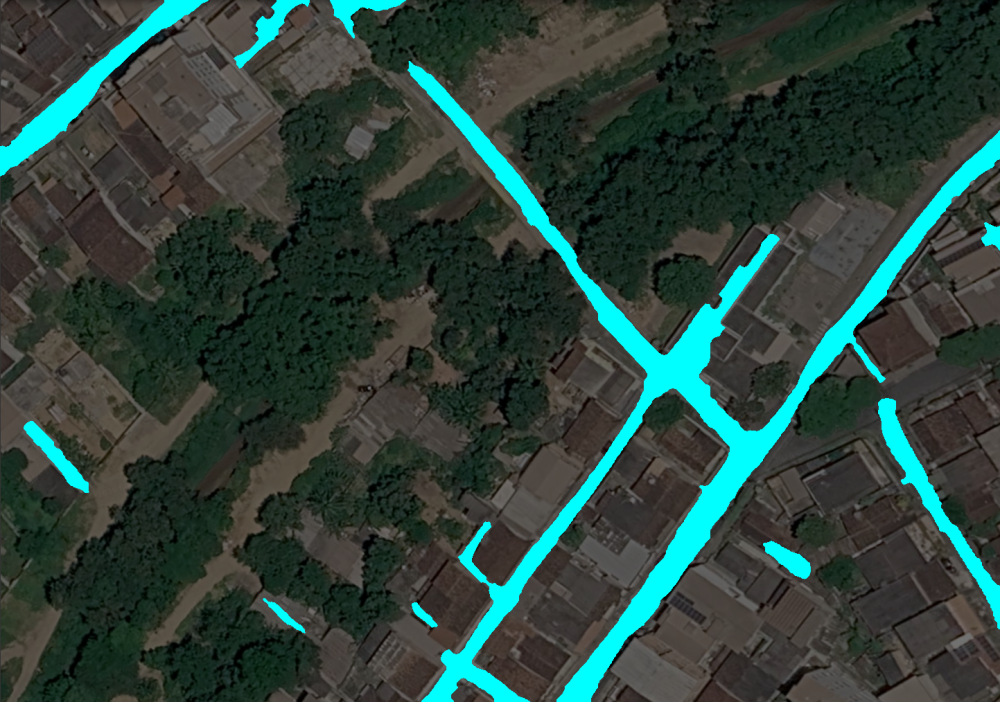
\includegraphics[width=\textwidth]{2026-05-12_151237_passo_6.png}
        \caption{Binária}
    \end{subfigure}\hfill
    \begin{subfigure}[b]{0.24\textwidth}
        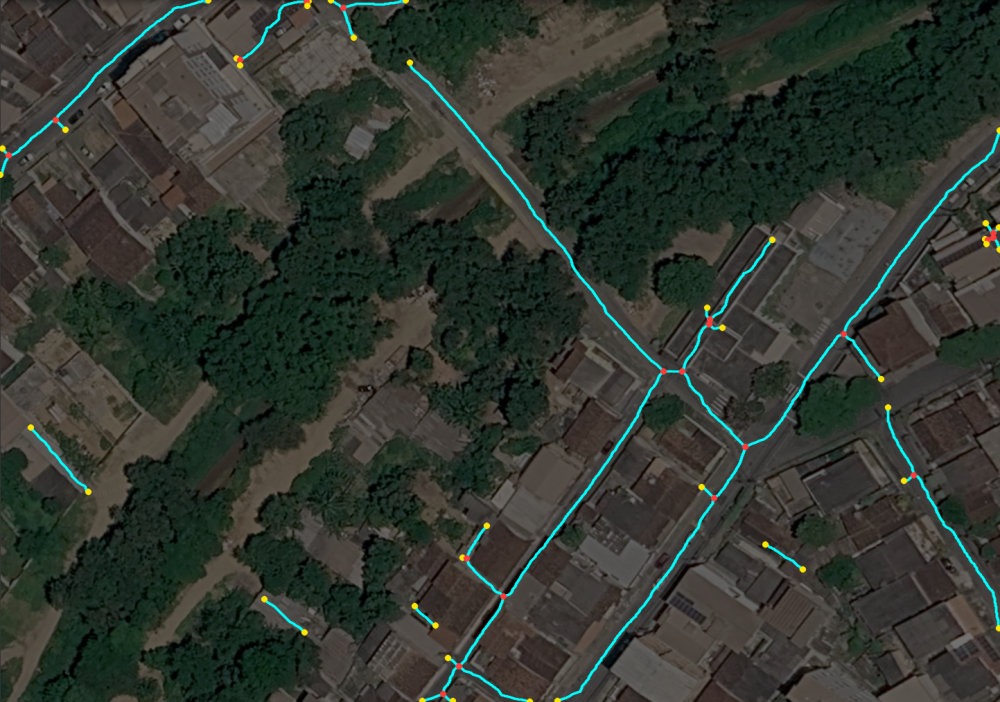
\includegraphics[width=\textwidth]{2026-05-12_151237_passo_7.png}
        \caption{Grafo Bruto}
    \end{subfigure}\hfill
    \begin{subfigure}[b]{0.24\textwidth}
        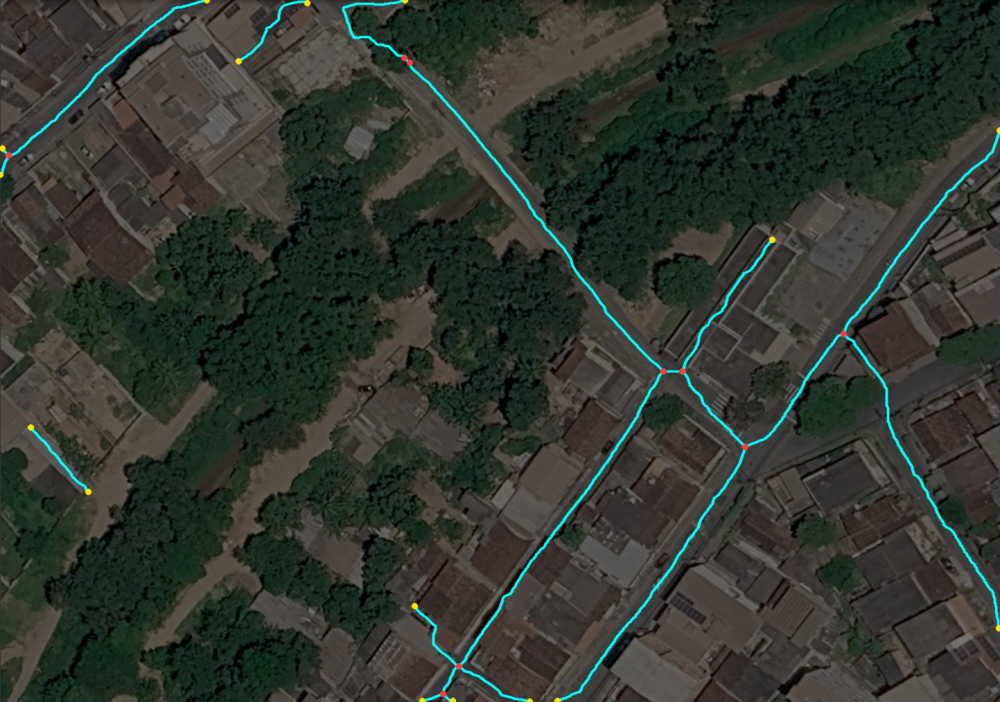
\includegraphics[width=\textwidth]{2026-05-12_151237_passo_8.png}
        \caption{Grafo Ref.}
    \end{subfigure}
    
    \vspace{0.15cm}
    \begin{subfigure}[b]{0.8\textwidth}
        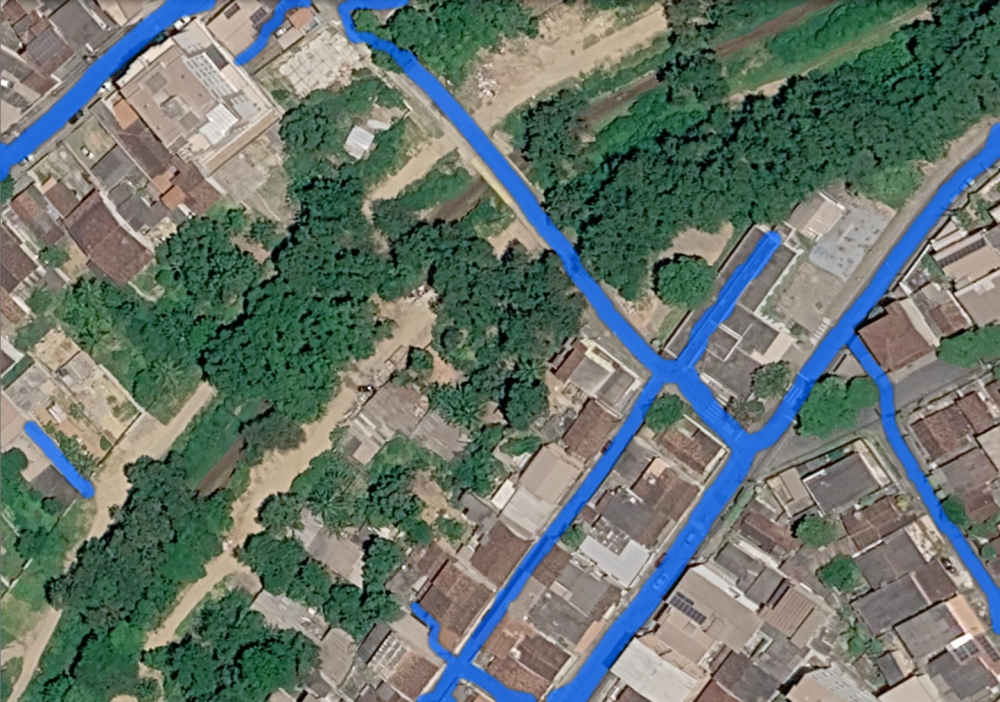
\includegraphics[width=\textwidth]{2026-05-12_151237_passo_9.png}
        \caption{Overlay final com pavimento classificado}
    \end{subfigure}
    \caption{Resultados do pipeline passo a passo para a imagem 151237 --- Favela em vale verde (área residencial com vegetação).}
    \label{fig:res_2026-05-12_151237}
\end{figure}

\begin{figure}[H]
    \centering
    \begin{subfigure}[b]{0.24\textwidth}
        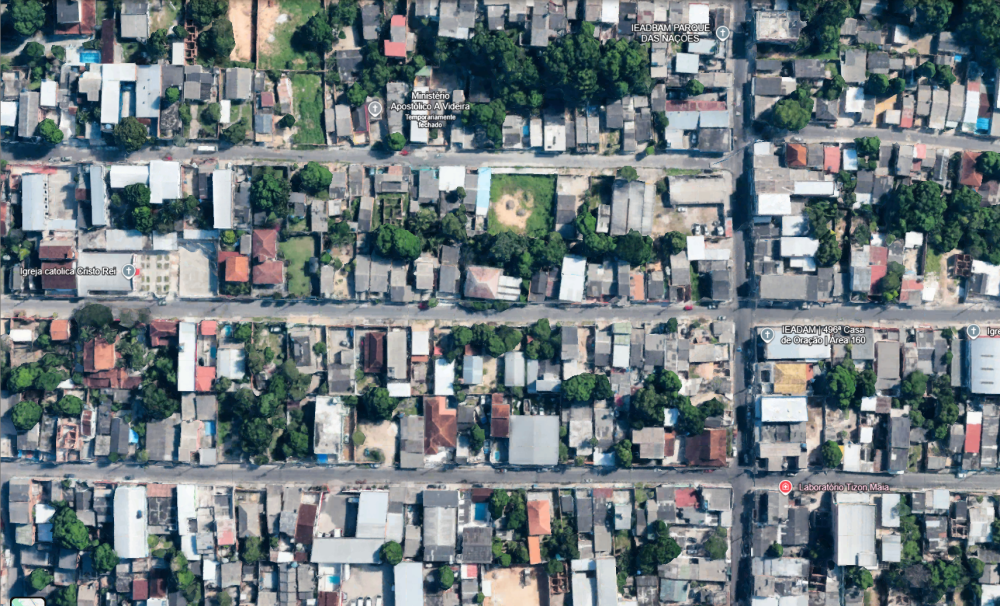
\includegraphics[width=\textwidth]{2026-05-13_020059_passo_1.png}
        \caption{Original}
    \end{subfigure}\hfill
    \begin{subfigure}[b]{0.24\textwidth}
        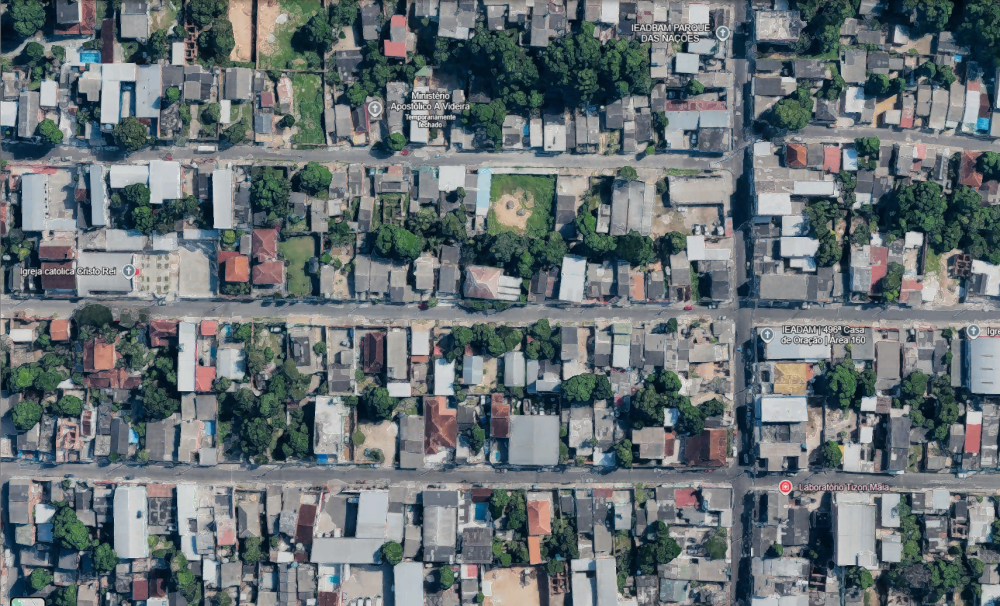
\includegraphics[width=\textwidth]{2026-05-13_020059_passo_2.png}
        \caption{Pré-proc.}
    \end{subfigure}\hfill
    \begin{subfigure}[b]{0.24\textwidth}
        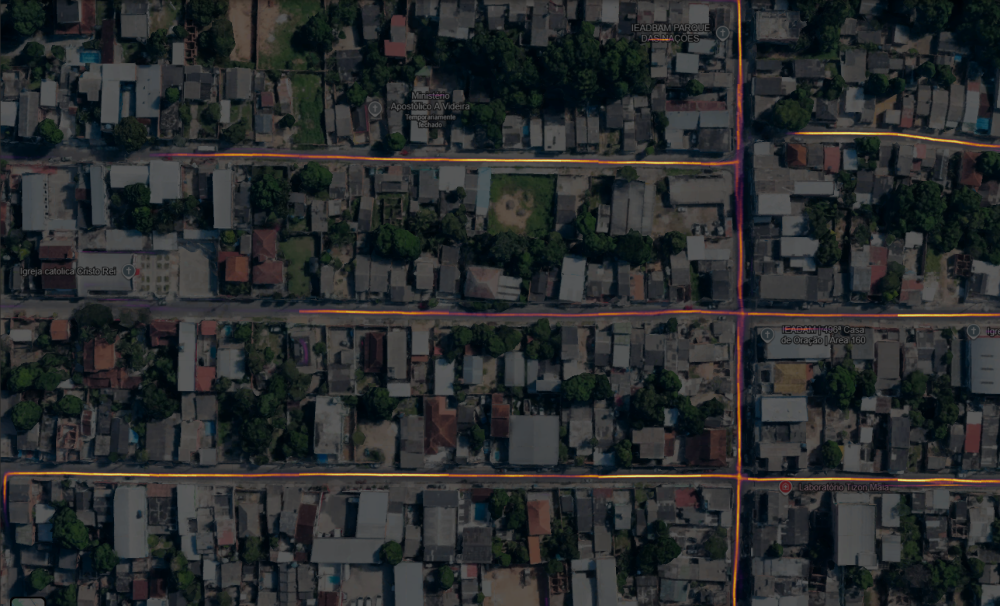
\includegraphics[width=\textwidth]{2026-05-13_020059_passo_3.png}
        \caption{Prob.\ Modelo}
    \end{subfigure}\hfill
    \begin{subfigure}[b]{0.24\textwidth}
        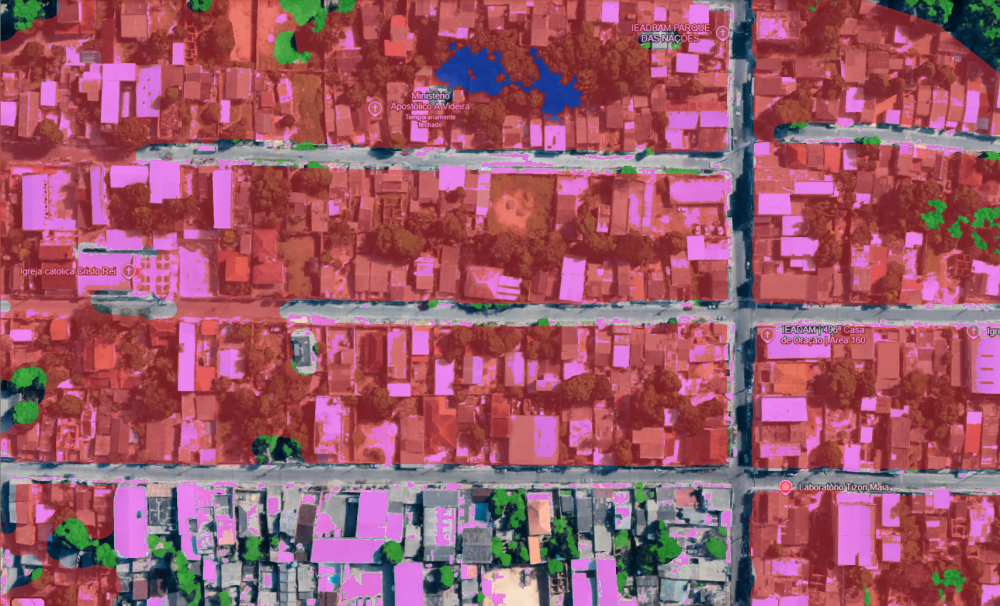
\includegraphics[width=\textwidth]{2026-05-13_020059_passo_4.png}
        \caption{Máscaras}
    \end{subfigure}
    
    \vspace{0.15cm}
    \begin{subfigure}[b]{0.24\textwidth}
        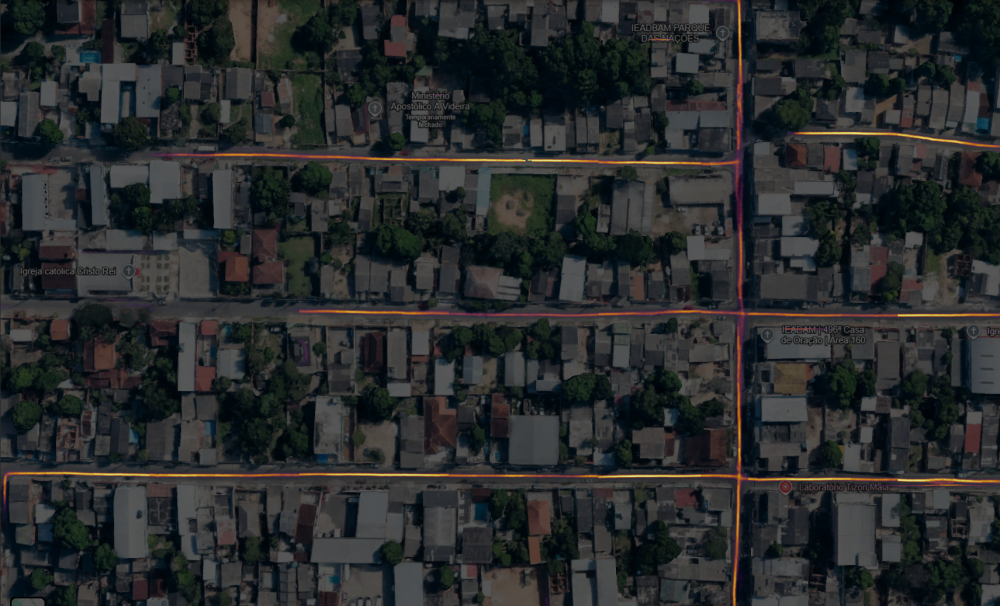
\includegraphics[width=\textwidth]{2026-05-13_020059_passo_5.png}
        \caption{Prob.\ Supr.}
    \end{subfigure}\hfill
    \begin{subfigure}[b]{0.24\textwidth}
        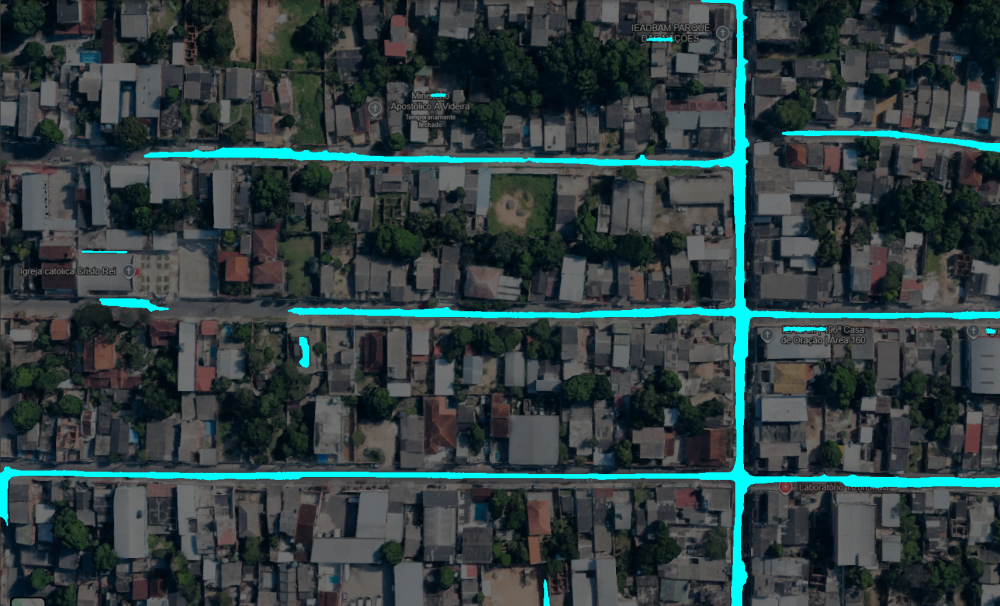
\includegraphics[width=\textwidth]{2026-05-13_020059_passo_6.png}
        \caption{Binária}
    \end{subfigure}\hfill
    \begin{subfigure}[b]{0.24\textwidth}
        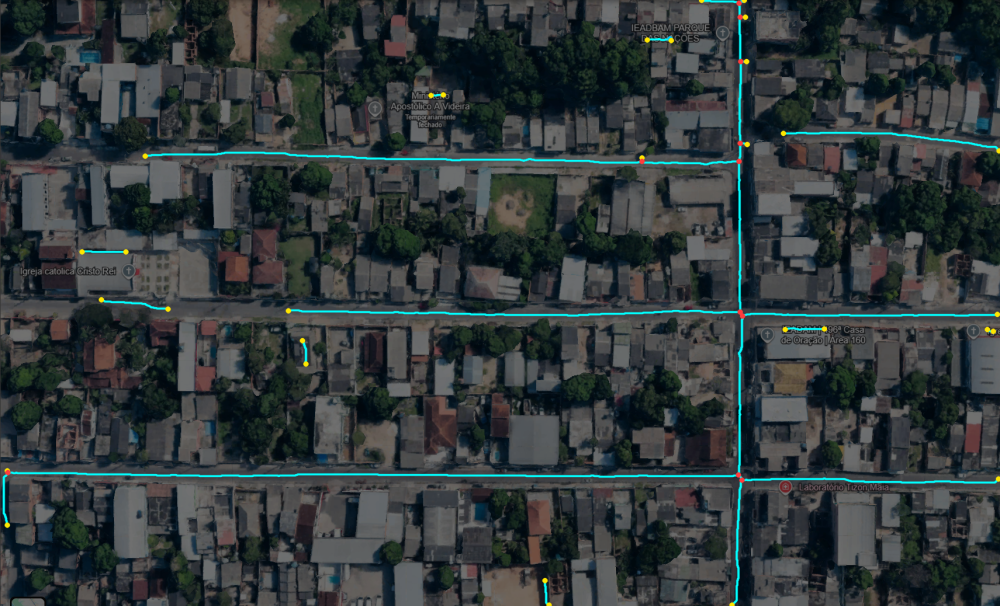
\includegraphics[width=\textwidth]{2026-05-13_020059_passo_7.png}
        \caption{Grafo Bruto}
    \end{subfigure}\hfill
    \begin{subfigure}[b]{0.24\textwidth}
        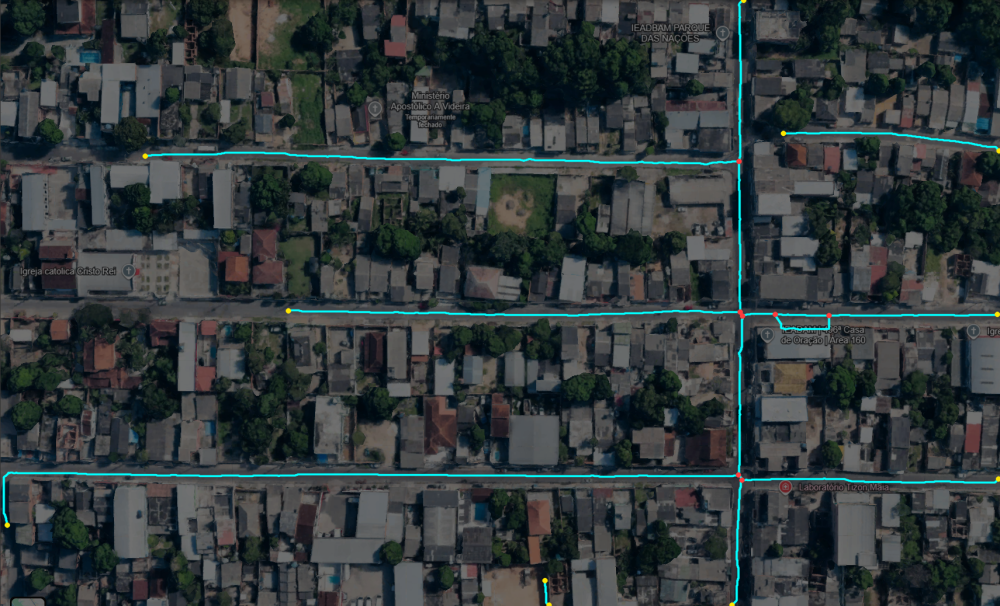
\includegraphics[width=\textwidth]{2026-05-13_020059_passo_8.png}
        \caption{Grafo Ref.}
    \end{subfigure}
    
    \vspace{0.15cm}
    \begin{subfigure}[b]{0.8\textwidth}
        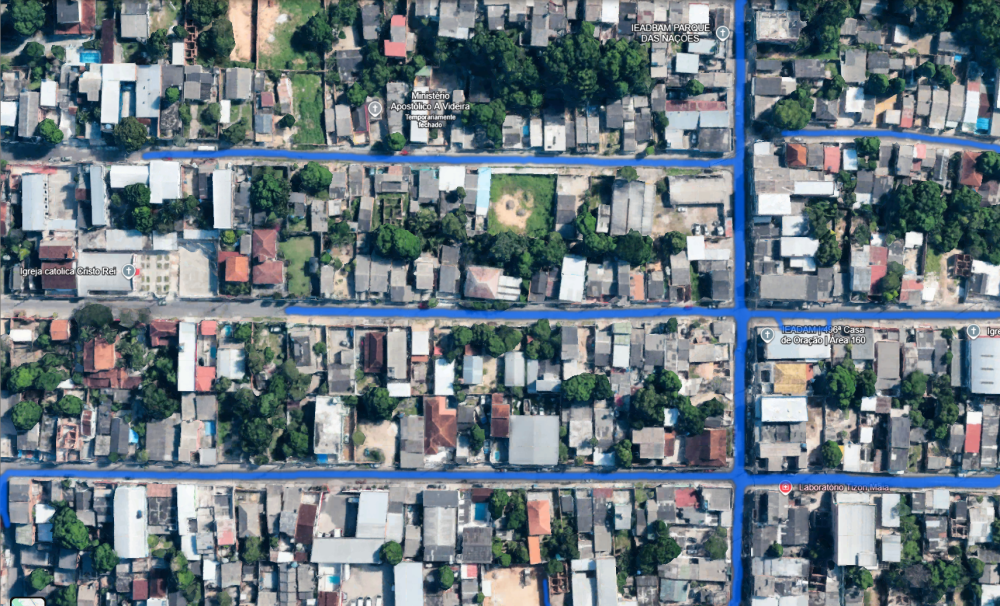
\includegraphics[width=\textwidth]{2026-05-13_020059_passo_9.png}
        \caption{Overlay final com pavimento classificado}
    \end{subfigure}
    \caption{Resultados do pipeline passo a passo para a imagem 020059 --- Urbano denso com vias longas paralelas.}
    \label{fig:res_2026-05-13_020059}
\end{figure}

\begin{figure}[H]
    \centering
    \begin{subfigure}[b]{0.24\textwidth}
        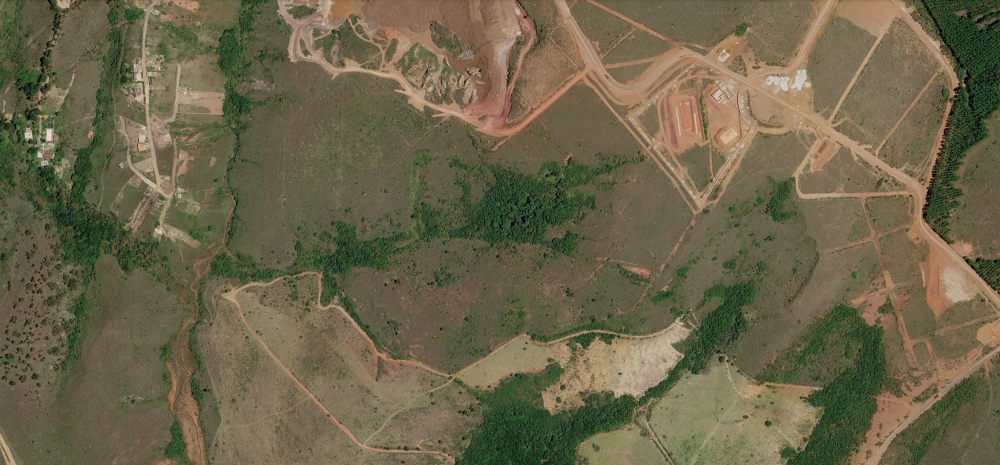
\includegraphics[width=\textwidth]{2026-05-16_165358_passo_1.png}
        \caption{Original}
    \end{subfigure}\hfill
    \begin{subfigure}[b]{0.24\textwidth}
        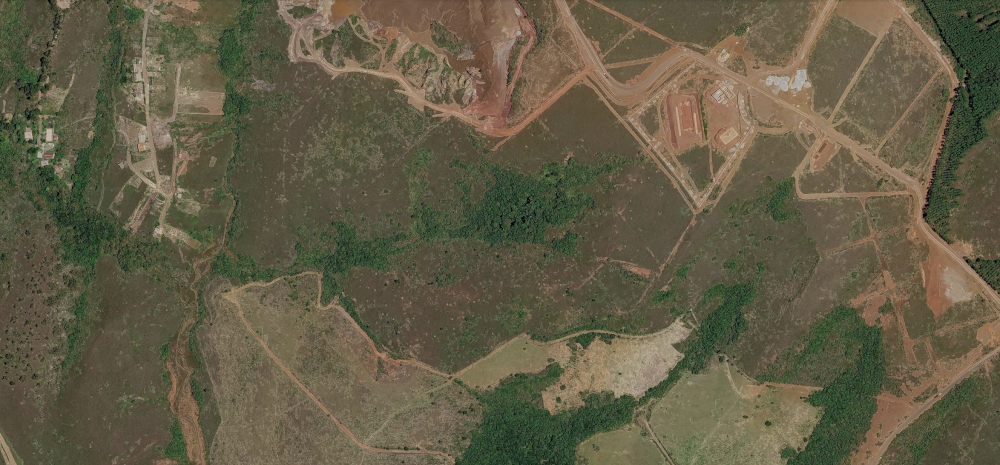
\includegraphics[width=\textwidth]{2026-05-16_165358_passo_2.png}
        \caption{Pré-proc.}
    \end{subfigure}\hfill
    \begin{subfigure}[b]{0.24\textwidth}
        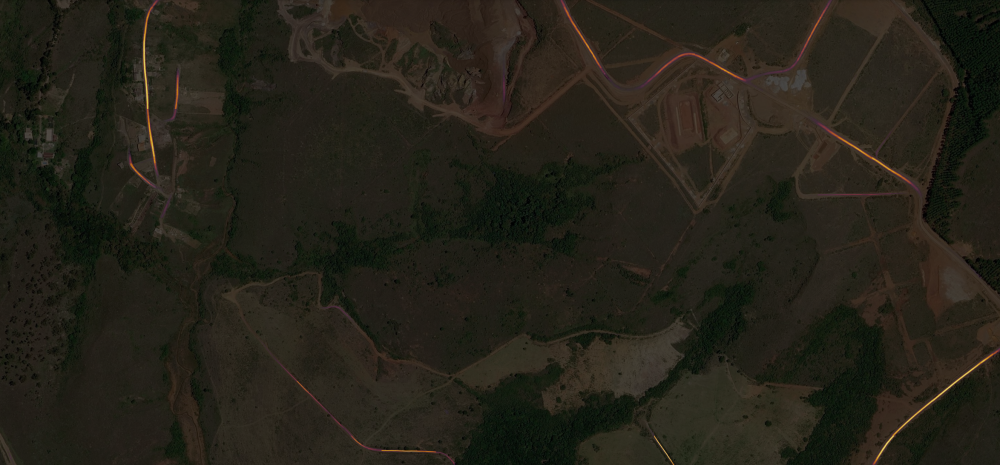
\includegraphics[width=\textwidth]{2026-05-16_165358_passo_3.png}
        \caption{Prob.\ Modelo}
    \end{subfigure}\hfill
    \begin{subfigure}[b]{0.24\textwidth}
        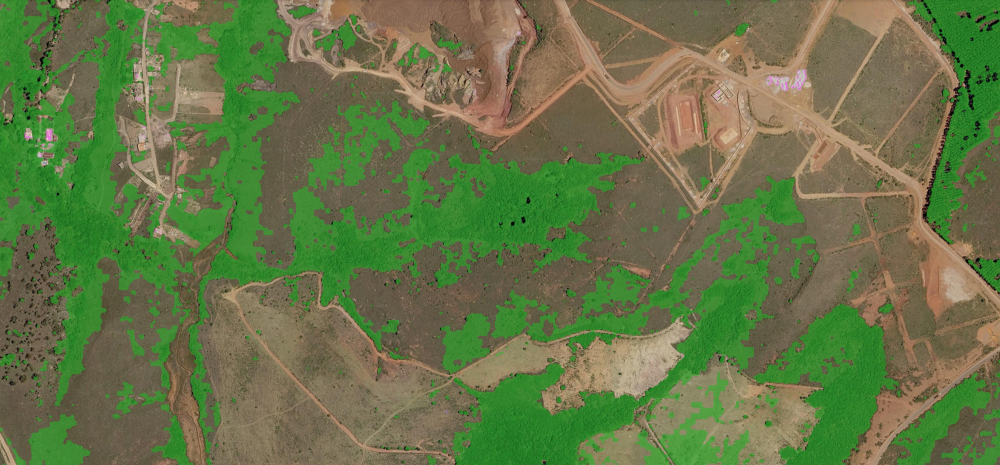
\includegraphics[width=\textwidth]{2026-05-16_165358_passo_4.png}
        \caption{Máscaras}
    \end{subfigure}
    
    \vspace{0.15cm}
    \begin{subfigure}[b]{0.24\textwidth}
        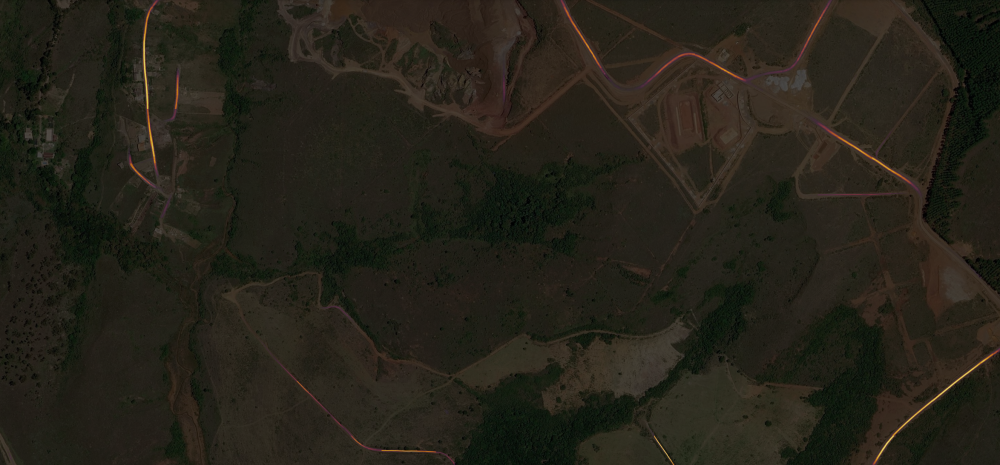
\includegraphics[width=\textwidth]{2026-05-16_165358_passo_5.png}
        \caption{Prob.\ Supr.}
    \end{subfigure}\hfill
    \begin{subfigure}[b]{0.24\textwidth}
        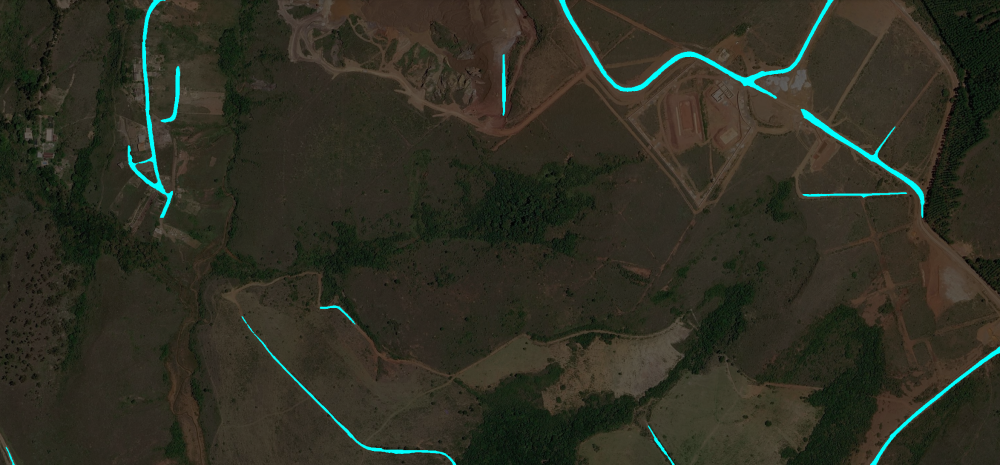
\includegraphics[width=\textwidth]{2026-05-16_165358_passo_6.png}
        \caption{Binária}
    \end{subfigure}\hfill
    \begin{subfigure}[b]{0.24\textwidth}
        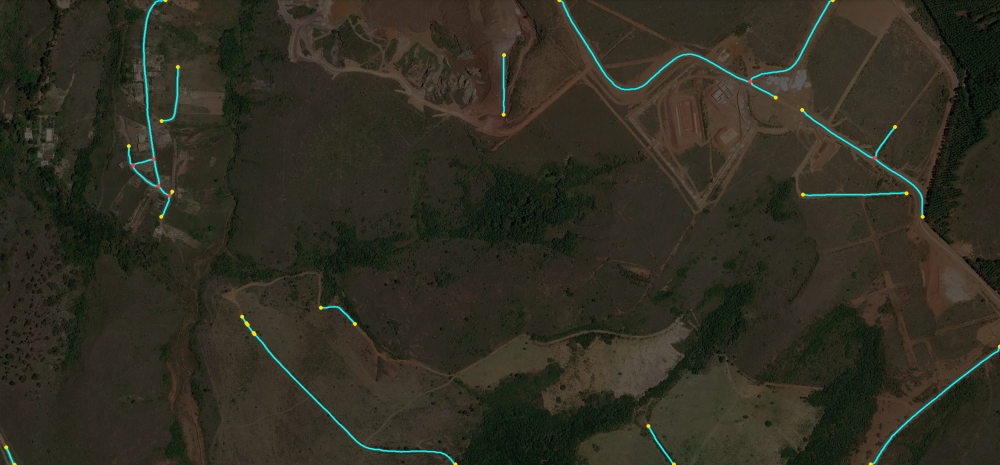
\includegraphics[width=\textwidth]{2026-05-16_165358_passo_7.png}
        \caption{Grafo Bruto}
    \end{subfigure}\hfill
    \begin{subfigure}[b]{0.24\textwidth}
        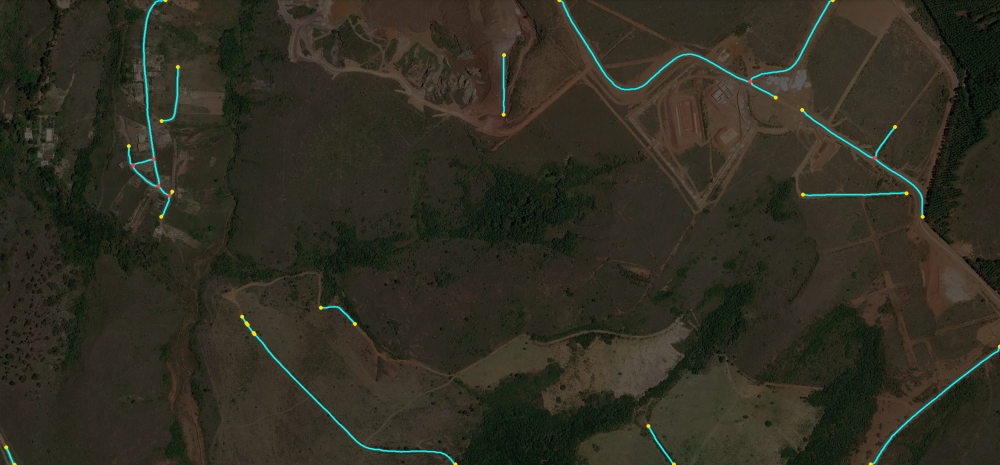
\includegraphics[width=\textwidth]{2026-05-16_165358_passo_8.png}
        \caption{Grafo Ref.}
    \end{subfigure}
    
    \vspace{0.15cm}
    \begin{subfigure}[b]{0.8\textwidth}
        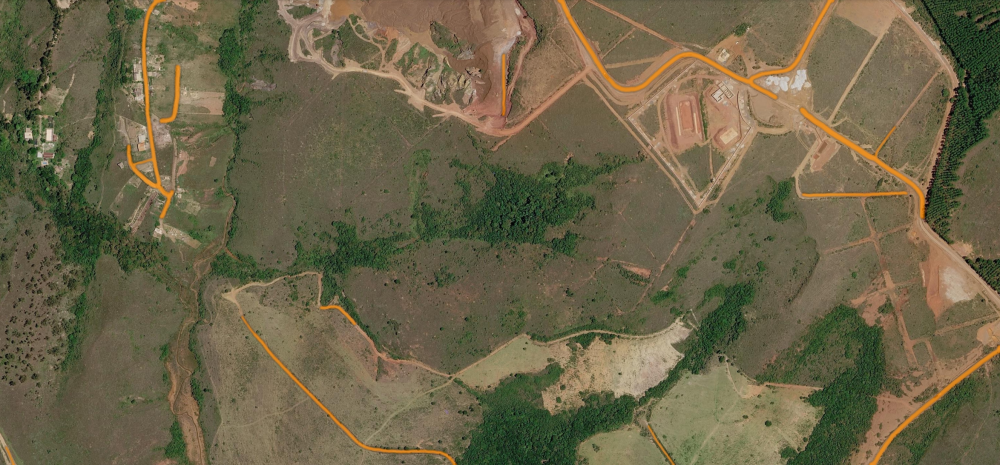
\includegraphics[width=\textwidth]{2026-05-16_165358_passo_9.png}
        \caption{Overlay final com pavimento classificado}
    \end{subfigure}
    \caption{Resultados do pipeline passo a passo para a imagem 165358 --- Rural com estradas de terra finas e sinuosas.}
    \label{fig:res_2026-05-16_165358}
\end{figure}

\begin{figure}[H]
    \centering
    \begin{subfigure}[b]{0.24\textwidth}
        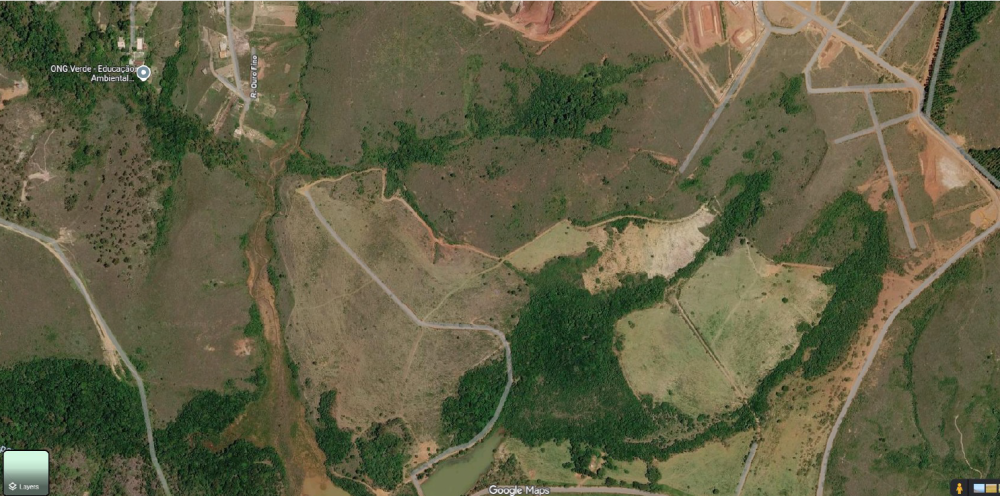
\includegraphics[width=\textwidth]{2026-05-11_202053_passo_1.png}
        \caption{Original}
    \end{subfigure}\hfill
    \begin{subfigure}[b]{0.24\textwidth}
        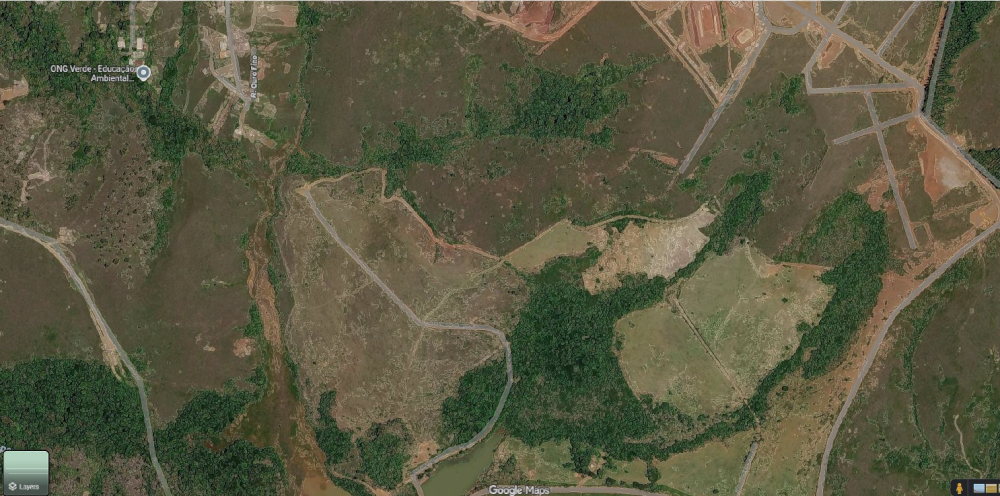
\includegraphics[width=\textwidth]{2026-05-11_202053_passo_2.png}
        \caption{Pré-proc.}
    \end{subfigure}\hfill
    \begin{subfigure}[b]{0.24\textwidth}
        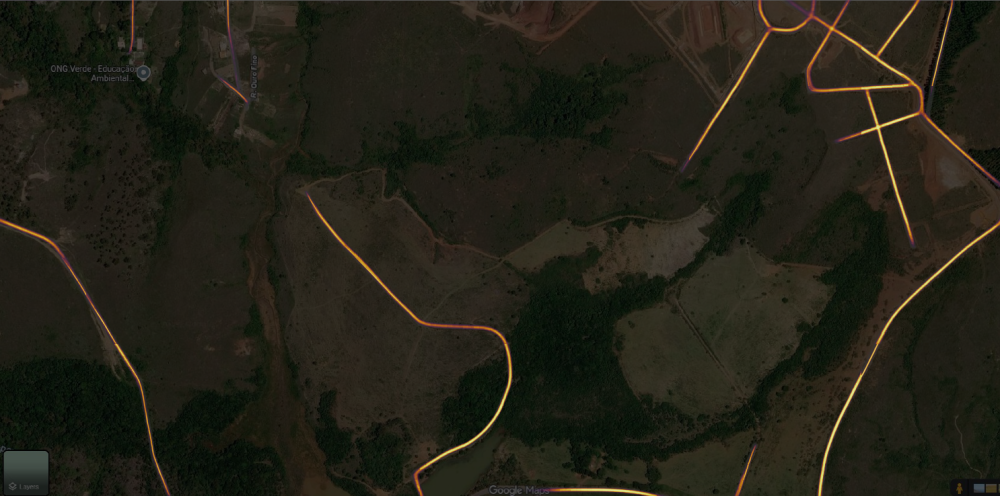
\includegraphics[width=\textwidth]{2026-05-11_202053_passo_3.png}
        \caption{Prob.\ Modelo}
    \end{subfigure}\hfill
    \begin{subfigure}[b]{0.24\textwidth}
        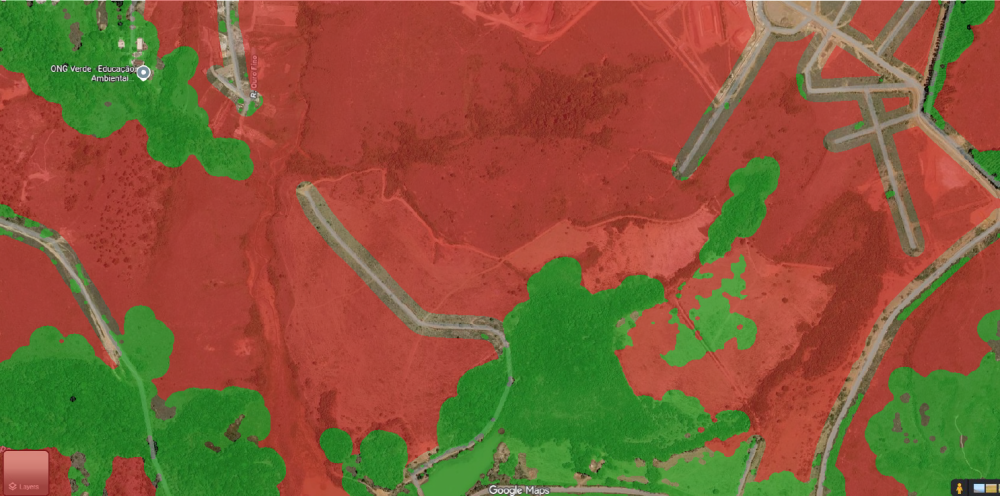
\includegraphics[width=\textwidth]{2026-05-11_202053_passo_4.png}
        \caption{Máscaras}
    \end{subfigure}
    
    \vspace{0.15cm}
    \begin{subfigure}[b]{0.24\textwidth}
        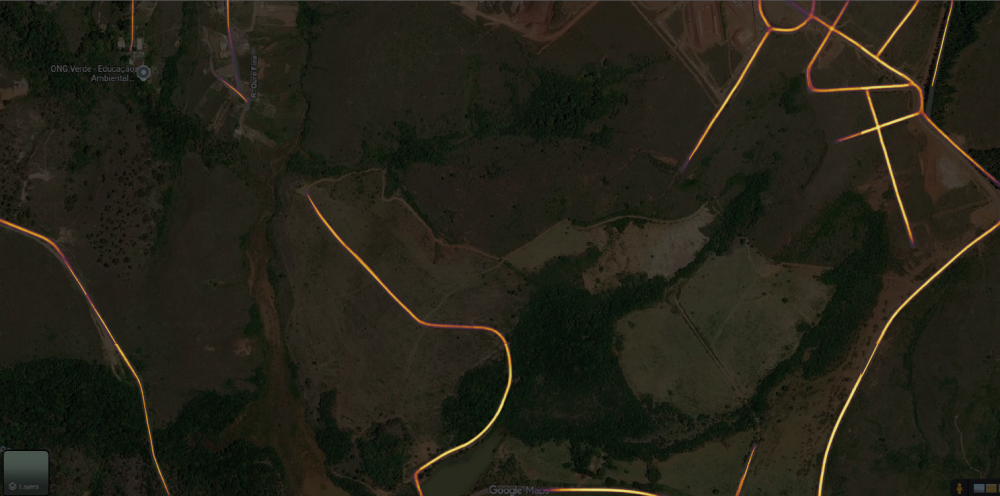
\includegraphics[width=\textwidth]{2026-05-11_202053_passo_5.png}
        \caption{Prob.\ Supr.}
    \end{subfigure}\hfill
    \begin{subfigure}[b]{0.24\textwidth}
        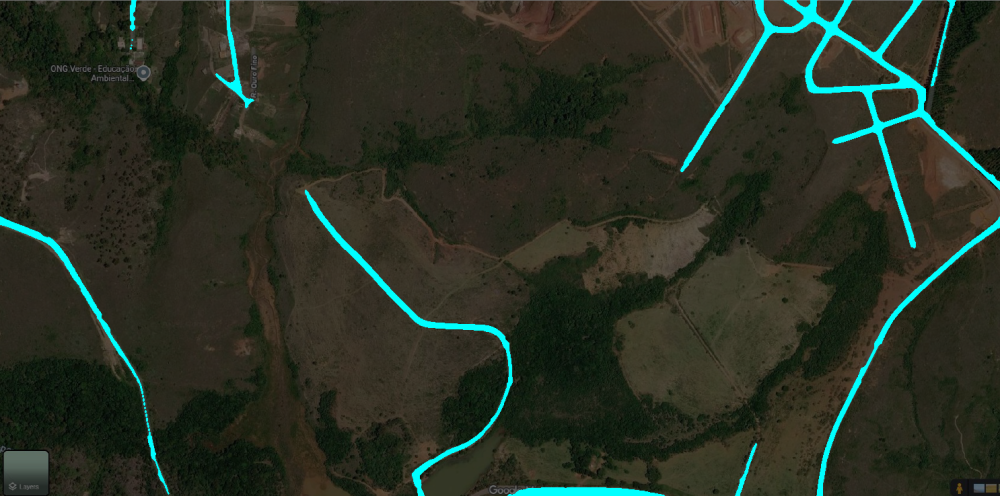
\includegraphics[width=\textwidth]{2026-05-11_202053_passo_6.png}
        \caption{Binária}
    \end{subfigure}\hfill
    \begin{subfigure}[b]{0.24\textwidth}
        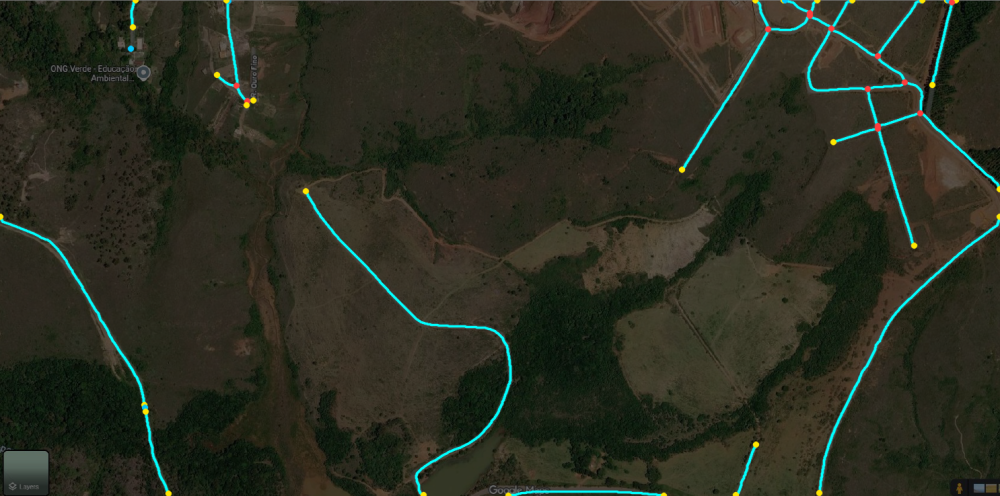
\includegraphics[width=\textwidth]{2026-05-11_202053_passo_7.png}
        \caption{Grafo Bruto}
    \end{subfigure}\hfill
    \begin{subfigure}[b]{0.24\textwidth}
        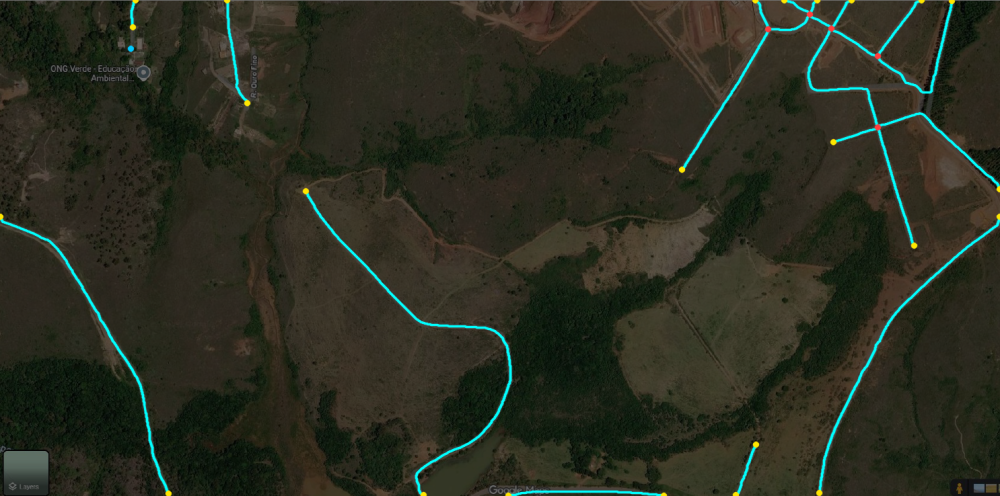
\includegraphics[width=\textwidth]{2026-05-11_202053_passo_8.png}
        \caption{Grafo Ref.}
    \end{subfigure}
    
    \vspace{0.15cm}
    \begin{subfigure}[b]{0.8\textwidth}
        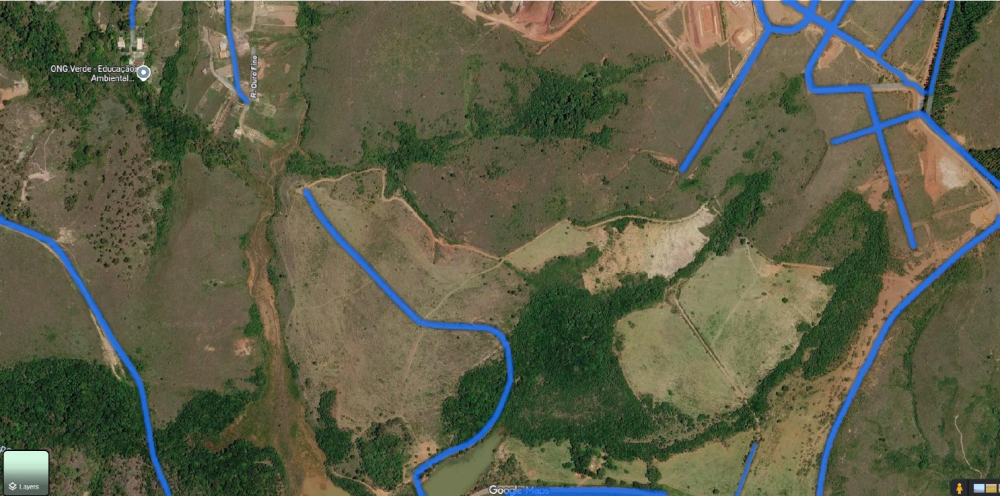
\includegraphics[width=\textwidth]{2026-05-11_202053_passo_9.png}
        \caption{Overlay final com pavimento classificado}
    \end{subfigure}
    \caption{Resultados do pipeline passo a passo para a imagem 202053 --- Imagem de satélite do PDF do professor (domínio rural).}
    \label{fig:res_2026-05-11_202053}
\end{figure}

\begin{figure}[H]
    \centering
    \begin{subfigure}[b]{0.24\textwidth}
        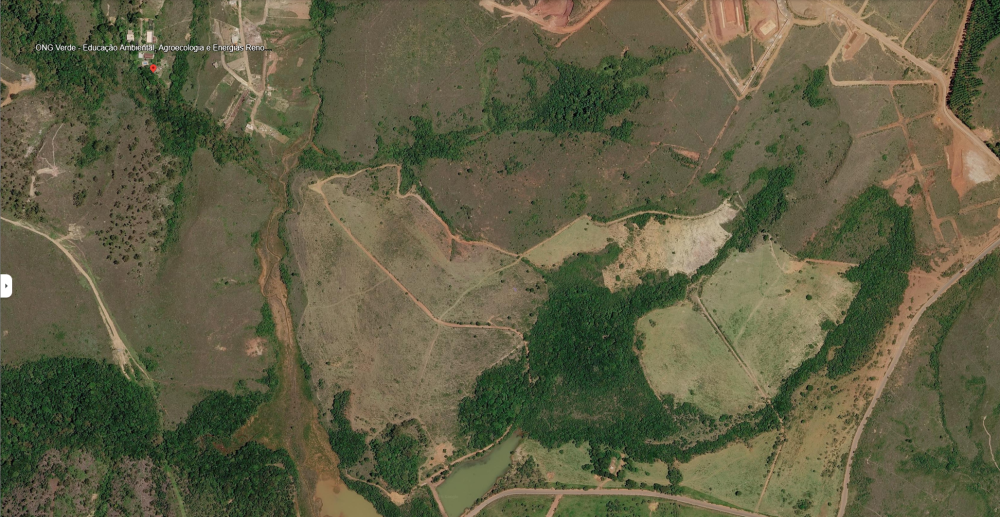
\includegraphics[width=\textwidth]{2026-06-14_131959_passo_1.png}
        \caption{Original}
    \end{subfigure}\hfill
    \begin{subfigure}[b]{0.24\textwidth}
        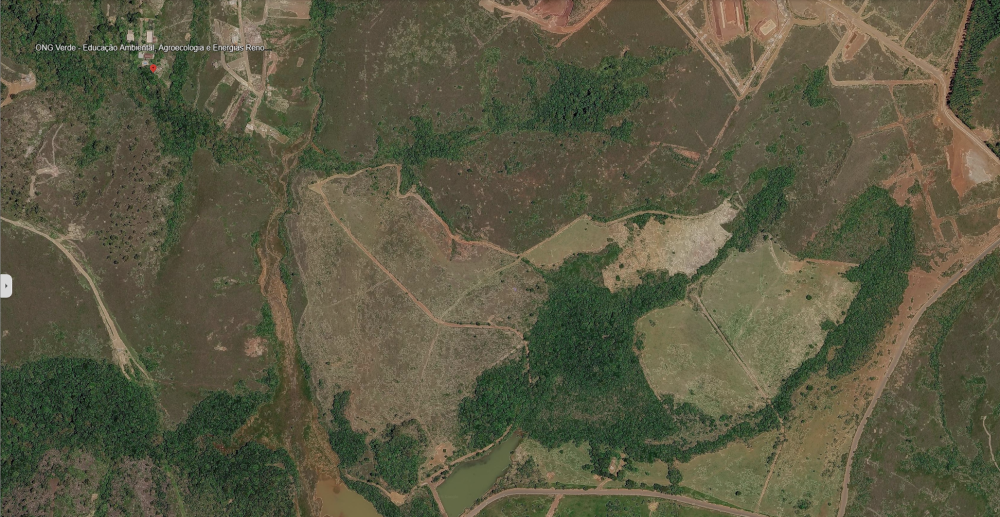
\includegraphics[width=\textwidth]{2026-06-14_131959_passo_2.png}
        \caption{Pré-proc.}
    \end{subfigure}\hfill
    \begin{subfigure}[b]{0.24\textwidth}
        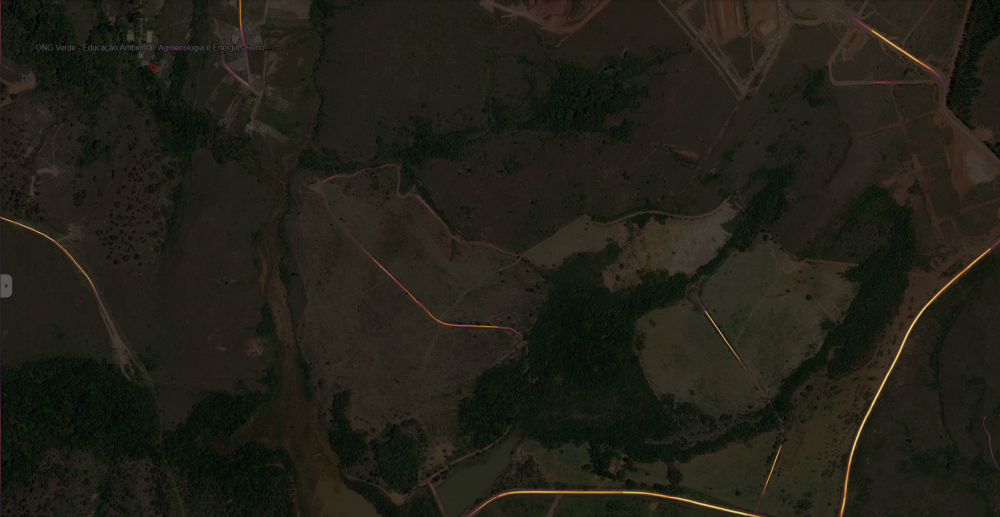
\includegraphics[width=\textwidth]{2026-06-14_131959_passo_3.png}
        \caption{Prob.\ Modelo}
    \end{subfigure}\hfill
    \begin{subfigure}[b]{0.24\textwidth}
        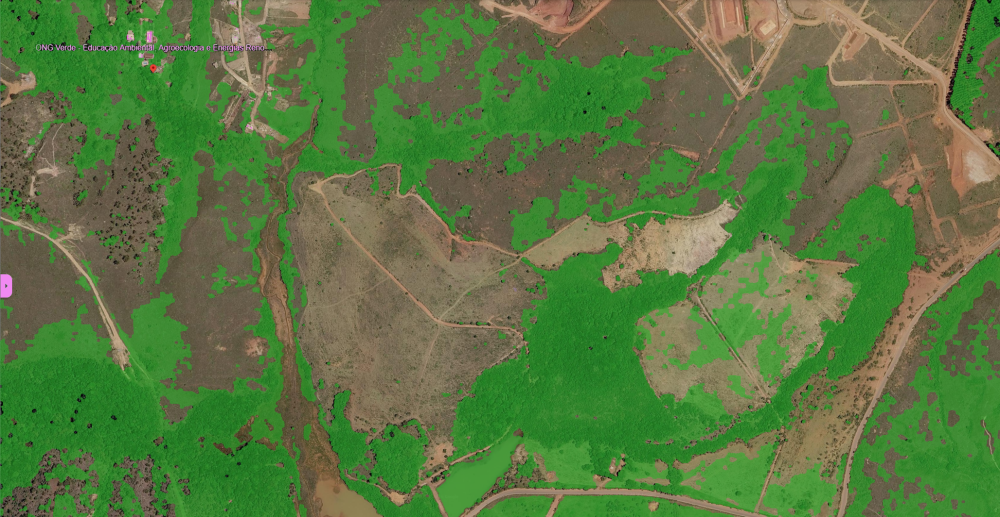
\includegraphics[width=\textwidth]{2026-06-14_131959_passo_4.png}
        \caption{Máscaras}
    \end{subfigure}
    
    \vspace{0.15cm}
    \begin{subfigure}[b]{0.24\textwidth}
        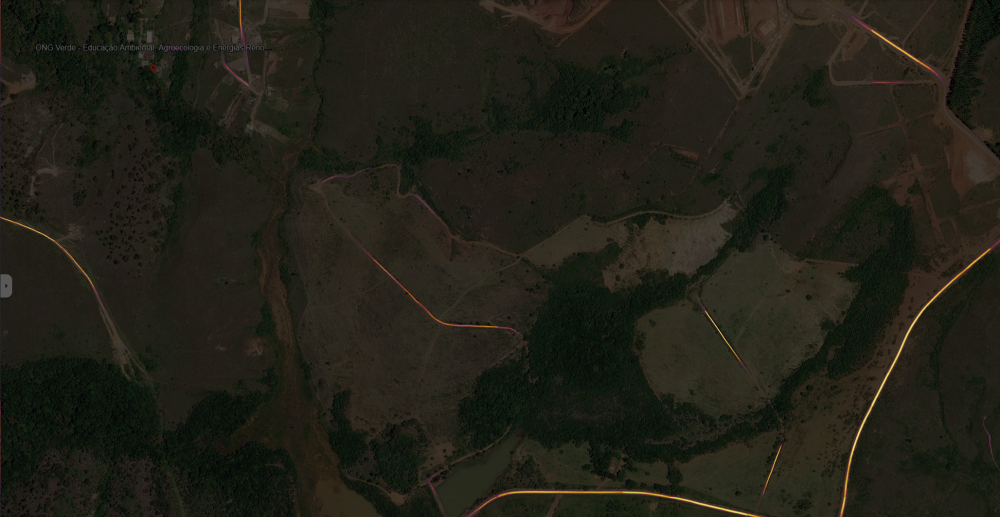
\includegraphics[width=\textwidth]{2026-06-14_131959_passo_5.png}
        \caption{Prob.\ Supr.}
    \end{subfigure}\hfill
    \begin{subfigure}[b]{0.24\textwidth}
        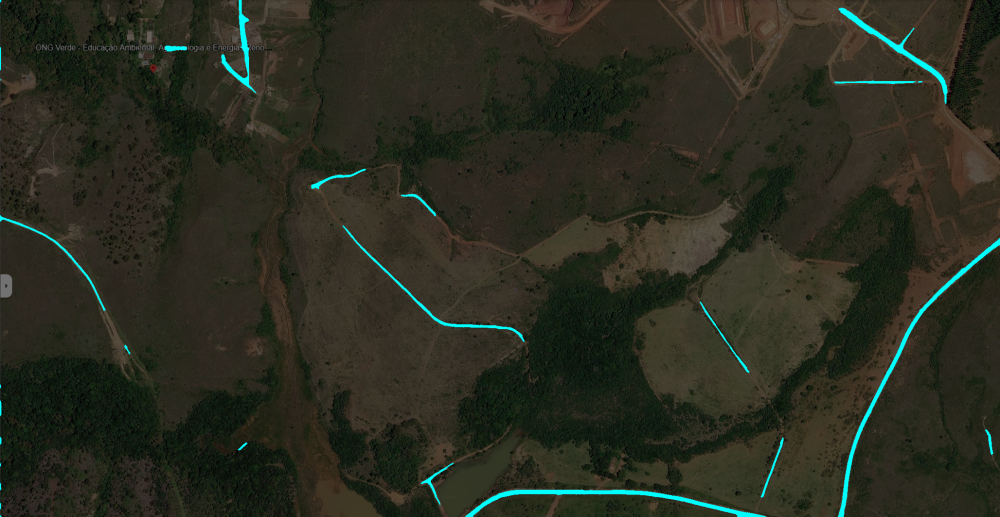
\includegraphics[width=\textwidth]{2026-06-14_131959_passo_6.png}
        \caption{Binária}
    \end{subfigure}\hfill
    \begin{subfigure}[b]{0.24\textwidth}
        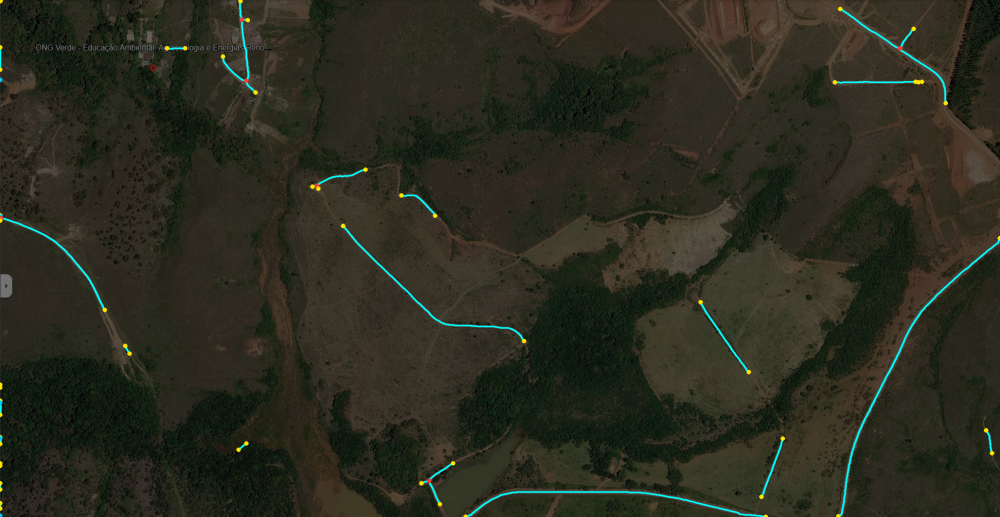
\includegraphics[width=\textwidth]{2026-06-14_131959_passo_7.png}
        \caption{Grafo Bruto}
    \end{subfigure}\hfill
    \begin{subfigure}[b]{0.24\textwidth}
        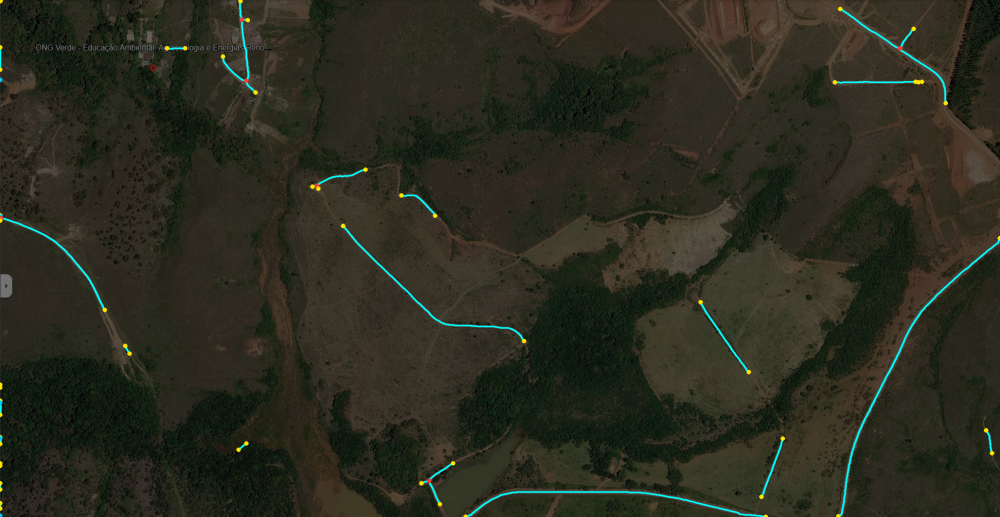
\includegraphics[width=\textwidth]{2026-06-14_131959_passo_8.png}
        \caption{Grafo Ref.}
    \end{subfigure}
    
    \vspace{0.15cm}
    \begin{subfigure}[b]{0.8\textwidth}
        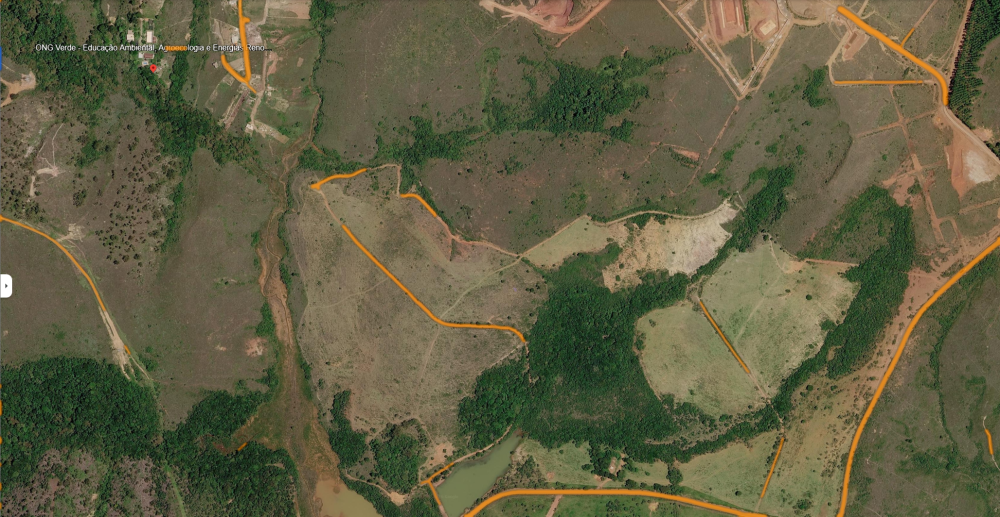
\includegraphics[width=\textwidth]{2026-06-14_131959_passo_9.png}
        \caption{Overlay final com pavimento classificado}
    \end{subfigure}
    \caption{Resultados do pipeline passo a passo para a imagem 131959 --- Rural com malha viária muito esparsa.}
    \label{fig:res_2026-06-14_131959}
\end{figure}

A máscara de contexto, exemplificada na Figura~\ref{fig:contexto}, é central para o desempenho: ela é o que distingue, por exemplo, um quarteirão de uma rua. Contudo, ela apresenta limitações sistemáticas. Um exemplo crítico ocorre no canto superior esquerdo da imagem \texttt{020059}: nas duas primeiras ruas horizontais paralelas, trechos da via são marcados erroneamente em vermelho (como quarteirão). Isso ocorre porque a confiança/probabilidade estimada pelo modelo SAM-Road nessas vias foi baixa, de modo que a etapa de recorte das ruas (\textit{carving}) não conseguiu subtrair a via da máscara de quarteirão. A similaridade espectral do asfalto claro/concreto com os telhados vizinhos agrava essa limitação, interrompendo a conectividade final do grafo nessas áreas. Essas limitações residuais (vermelho sobre trechos de rua de baixa probabilidade, telhado de cor atípica não reconhecido) explicam os casos ``média/boa'' da Tabela~\ref{tab:resumo}.

\begin{figure}[H]
    \centering
    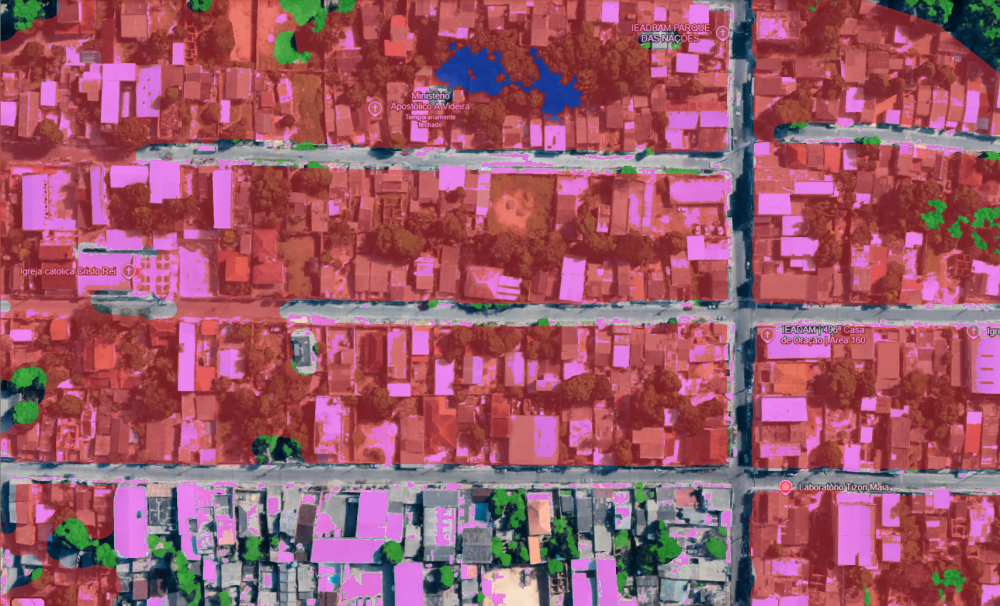
\includegraphics[width=0.85\textwidth]{contexto_legenda.png}
    \caption{Máscara de contexto (cores da Tabela 1): vermelho = quarteirão, verde = vegetação, rosa = via clara rejeitada. As ruas detectadas são recortadas do vermelho.}
    \label{fig:contexto}
\end{figure}

\section{Limitações e Trabalhos Futuros}
\label{sec:futuro}

\begin{itemize}
    \item \textbf{Recall em rural}: o modelo perde estradas de terra muito
    fracas (ex.: 131959, 165358), deixando vias sem marcar. A alavanca
    imediata é baixar \texttt{--limiar-via}; o ganho estrutural viria do
    ajuste fino.
    \item \textbf{Ajuste fino não realizado}: por falta de GPU e pelo
    limite de $\sim$4\,h do Colab gratuito. O dataset e os \textit{scripts} estão
    prontos; é o próximo passo natural.
    \item \textbf{Terra clara $\times$ asfalto cinza}: difícil de separar só com
    RGB; a solução robusta é uma cabeça de superfície supervisionada usando o
    atributo pavimentado (paved) do SpaceNet.
    \item \textbf{Máscara de telhado}: pode marcar vermelho sobre trechos de
    rua de baixa probabilidade (020059) ou não reconhecer telhados de cor
    atípica (151237).
\end{itemize}

\section{Conclusão}

Desenvolvemos um sistema completo e robusto que detecta vias, classifica o
pavimento, sobrepõe o resultado e reconstrói a malha como grafo conectado,
funcionando de forma adaptativa em diferentes domínios (urbano denso, favela,
rural) sem ajuste manual por imagem. O pós-processamento topológico em
grafo e as máscaras de contexto foram decisivos para a qualidade
(F1 de $0{,}751$ para $0{,}909$). As falhas residuais concentram-se no
recall de estradas de terra fracas e na ambiguidade de cores, ambas
endereçáveis por ajuste fino --- não realizado aqui apenas por
restrições de hardware.

\section*{Código e Pesos}

O código fonte deste projeto está disponível no repositório GitHub:
\begin{center}
\url{https://github.com/felcoslop/TP_RP}
\end{center}

Os pesos pré-treinados ($\sim$1\,GB cada) não acompanham o repositório devido a limitações de tamanho de arquivo. Faça o download dos pesos e coloque-os na pasta \texttt{weights/} conforme as instruções do repositório:
\begin{center}
\url{https://drive.google.com/file/d/1e6AJ6tSdS1dVmAF4KuOcWVLpn5_opASH/view?usp=drive_link}
\end{center}


\begin{thebibliography}{9}
\bibitem{samroad} C. Hetang \textit{et al.}, ``Segment Anything Model for Road Network Graph Extraction,'' \textit{CVPRW}, 2024.
\bibitem{samroadpp} Z. Yin \textit{et al.}, ``Towards Satellite Image Road Graph Extraction: A Global-Scale Dataset and A Novel Method,'' \textit{CVPR}, 2025.
\bibitem{sam} A. Kirillov \textit{et al.}, ``Segment Anything,'' \textit{ICCV}, 2023.
\bibitem{cldice} S. Shit \textit{et al.}, ``clDice --- a Novel Topology-Preserving Loss Function for Tubular Structure Segmentation,'' \textit{CVPR}, 2021.
\bibitem{spacenet} SpaceNet Roads Challenge, \textit{spacenet.ai}, 2018.
\end{thebibliography}

\end{document}
